% CERTA: the paper. Original Paper, laid out after Bioinformatics (OUP) for
% review; the journal's own class is applied at acceptance.
% Build: python make_numbers.py && python make_figures.py && latexmk -pdf main.tex
\documentclass[11pt]{article}
\usepackage[a4paper,margin=25mm]{geometry}
\usepackage{amsmath,amssymb,amsthm}
\usepackage{mathptmx}
\usepackage[T1]{fontenc}
\usepackage{microtype}
\usepackage{graphicx}
\usepackage{booktabs}
\usepackage{multirow}
\usepackage{xcolor}
\usepackage[round,authoryear]{natbib}
\usepackage[labelfont=bf,font=small]{caption}
\usepackage{enumitem}
\usepackage{tikz}
\usetikzlibrary{positioning,arrows.meta,fit}
\usepackage{lineno}
\usepackage[hidelinks]{hyperref}
\usepackage{authblk}

% Generated by make_numbers.py from bench/results/; do not edit.
\newcommand{\AqAfter}{96.29}% aim1_2026-10/summary.tsv
\newcommand{\AqAfterMax}{96.83}% aim1_2026-10/summary.tsv
\newcommand{\AqBase}{95.65}% aim1_2026-10/summary.tsv
\newcommand{\AqMs}{0.272}% aim1_2026-10/summary.tsv
\newcommand{\BenchReads}{20,001,073}% hg002_2026-09/galaxy_timing_v06.tsv
\newcommand{\CkFaultKinds}{8}% aim4_pr_2026-10/tamper_hg002.tsv
\newcommand{\CkFaults}{24,306}% aim4_pr_2026-10/tamper_hg002.tsv
\newcommand{\CkRecords}{8,000,000}% aim4_pr_2026-10/check_hg00{2,5}_2M.log
\newcommand{\CkRejected}{24,306}% aim4_pr_2026-10/tamper_hg002.tsv
\newcommand{\CkUsHi}{232}% aim4_pr_2026-10/check_hg00{2,5}_2M.log
\newcommand{\CkUsLo}{182}% aim4_pr_2026-10/check_hg00{2,5}_2M.log
\newcommand{\CkXS}{303,682}% aim4_pr_2026-10/check_hg00{2,5}_2M.log
\newcommand{\CpuTierCert}{94.38}% hg002_2026-10/{galaxy,a2}_cpu_tier.stats.json
\newcommand{\FAPBwaCfg}{-}% hg002_2026-10/final_a2.tsv
\newcommand{\FAPBwaCpu}{13,902}% hg002_2026-10/final_a2.tsv
\newcommand{\FAPBwaSys}{100}% hg002_2026-10/final_a2.tsv
\newcommand{\FAPBwaWall}{256.35}% hg002_2026-10/final_a2.tsv
\newcommand{\FAPBwaXMini}{0.31}% hg002_2026-10/final_a2.tsv
\newcommand{\FAPCpuIvCfg}{64}% hg002_2026-10/final_a2.tsv
\newcommand{\FAPCpuIvCpu}{2,145}% hg002_2026-10/final_a2.tsv
\newcommand{\FAPCpuIvSys}{11}% hg002_2026-10/final_a2.tsv
\newcommand{\FAPCpuIvWall}{36.73}% hg002_2026-10/final_a2.tsv
\newcommand{\FAPCpuIvXBwa}{7.0}% hg002_2026-10/final_a2.tsv
\newcommand{\FAPCpuIvXMini}{2.14}% hg002_2026-10/final_a2.tsv
\newcommand{\FAPCpuKdCfg}{64:64}% hg002_2026-10/final_a2.tsv
\newcommand{\FAPCpuKdCpu}{3,219}% hg002_2026-10/final_a2.tsv
\newcommand{\FAPCpuKdSys}{39}% hg002_2026-10/final_a2.tsv
\newcommand{\FAPCpuKdWall}{59.70}% hg002_2026-10/final_a2.tsv
\newcommand{\FAPCpuKdXBwa}{4.3}% hg002_2026-10/final_a2.tsv
\newcommand{\FAPCpuKdXMini}{1.32}% hg002_2026-10/final_a2.tsv
\newcommand{\FAPCpuKtCfg}{64:64}% hg002_2026-10/final_a2.tsv
\newcommand{\FAPCpuKtCpu}{3,234}% hg002_2026-10/final_a2.tsv
\newcommand{\FAPCpuKtSys}{24}% hg002_2026-10/final_a2.tsv
\newcommand{\FAPCpuKtWall}{56.27}% hg002_2026-10/final_a2.tsv
\newcommand{\FAPCpuKtXBwa}{4.6}% hg002_2026-10/final_a2.tsv
\newcommand{\FAPCpuKtXMini}{1.40}% hg002_2026-10/final_a2.tsv
\newcommand{\FAPMiniCfg}{-}% hg002_2026-10/final_a2.tsv
\newcommand{\FAPMiniCpu}{3,965}% hg002_2026-10/final_a2.tsv
\newcommand{\FAPMiniSys}{27}% hg002_2026-10/final_a2.tsv
\newcommand{\FAPMiniWall}{78.72}% hg002_2026-10/final_a2.tsv
\newcommand{\FAPMiniXBwa}{3.3}% hg002_2026-10/final_a2.tsv
\newcommand{\FASBtCfg}{-}% hg002_2026-10/final_a2.tsv
\newcommand{\FASBtCpu}{9,945}% hg002_2026-10/final_a2.tsv
\newcommand{\FASBtSys}{8}% hg002_2026-10/final_a2.tsv
\newcommand{\FASBtWall}{159.31}% hg002_2026-10/final_a2.tsv
\newcommand{\FASBtXBwa}{0.7}% hg002_2026-10/final_a2.tsv
\newcommand{\FASBtXMini}{0.23}% hg002_2026-10/final_a2.tsv
\newcommand{\FASBwaCfg}{-}% hg002_2026-10/final_a2.tsv
\newcommand{\FASBwaCpu}{5,195}% hg002_2026-10/final_a2.tsv
\newcommand{\FASBwaSys}{65}% hg002_2026-10/final_a2.tsv
\newcommand{\FASBwaWall}{110.64}% hg002_2026-10/final_a2.tsv
\newcommand{\FASBwaXMini}{0.33}% hg002_2026-10/final_a2.tsv
\newcommand{\FASCpuCfg}{64:64}% hg002_2026-10/final_a2.tsv
\newcommand{\FASCpuCpu}{1,170}% hg002_2026-10/final_a2.tsv
\newcommand{\FASCpuIvCfg}{64}% hg002_2026-10/final_a2.tsv
\newcommand{\FASCpuIvCpu}{1,035}% hg002_2026-10/final_a2.tsv
\newcommand{\FASCpuIvSys}{7}% hg002_2026-10/final_a2.tsv
\newcommand{\FASCpuIvWall}{17.98}% hg002_2026-10/final_a2.tsv
\newcommand{\FASCpuIvXBwa}{6.2}% hg002_2026-10/final_a2.tsv
\newcommand{\FASCpuIvXMini}{2.02}% hg002_2026-10/final_a2.tsv
\newcommand{\FASCpuSys}{17}% hg002_2026-10/final_a2.tsv
\newcommand{\FASCpuTierCfg}{64}% hg002_2026-10/final_a2.tsv
\newcommand{\FASCpuTierCpu}{439}% hg002_2026-10/final_a2.tsv
\newcommand{\FASCpuTierSys}{6}% hg002_2026-10/final_a2.tsv
\newcommand{\FASCpuTierWall}{8.61}% hg002_2026-10/final_a2.tsv
\newcommand{\FASCpuTierXBwa}{12.9}% hg002_2026-10/final_a2.tsv
\newcommand{\FASCpuTierXMini}{4.22}% hg002_2026-10/final_a2.tsv
\newcommand{\FASCpuWall}{19.82}% hg002_2026-10/final_a2.tsv
\newcommand{\FASCpuXBwa}{5.6}% hg002_2026-10/final_a2.tsv
\newcommand{\FASCpuXMini}{1.83}% hg002_2026-10/final_a2.tsv
\newcommand{\FASMiniCfg}{-}% hg002_2026-10/final_a2.tsv
\newcommand{\FASMiniCpu}{1,551}% hg002_2026-10/final_a2.tsv
\newcommand{\FASMiniSys}{16}% hg002_2026-10/final_a2.tsv
\newcommand{\FASMiniWall}{36.32}% hg002_2026-10/final_a2.tsv
\newcommand{\FASMiniXBwa}{3.0}% hg002_2026-10/final_a2.tsv
\newcommand{\FASMmCfg}{-}% hg002_2026-10/final_a2.tsv
\newcommand{\FASMmCpu}{3,659}% hg002_2026-10/final_a2.tsv
\newcommand{\FASMmSys}{22}% hg002_2026-10/final_a2.tsv
\newcommand{\FASMmWall}{94.70}% hg002_2026-10/final_a2.tsv
\newcommand{\FASMmXBwa}{1.2}% hg002_2026-10/final_a2.tsv
\newcommand{\FASMmXMini}{0.38}% hg002_2026-10/final_a2.tsv
\newcommand{\FASStrobeCfg}{-}% hg002_2026-10/final_a2.tsv
\newcommand{\FASStrobeCpu}{983}% hg002_2026-10/final_a2.tsv
\newcommand{\FASStrobeSys}{39}% hg002_2026-10/final_a2.tsv
\newcommand{\FASStrobeWall}{61.87}% hg002_2026-10/final_a2.tsv
\newcommand{\FASStrobeXBwa}{1.8}% hg002_2026-10/final_a2.tsv
\newcommand{\FASStrobeXMini}{0.59}% hg002_2026-10/final_a2.tsv
\newcommand{\FCAPDefCpuCpu}{2,138}% hg002_2026-10/full_cert_a2.tsv
\newcommand{\FCAPDefCpuRss}{21.4}% hg002_2026-10/full_cert_a2.tsv
\newcommand{\FCAPDefCpuWall}{36.68}% hg002_2026-10/full_cert_a2.tsv
\newcommand{\FCAPDefCpuXBwa}{7.0}% hg002_2026-10/full_cert_a2.tsv
\newcommand{\FCAPDefCpuXMini}{2.15}% hg002_2026-10/full_cert_a2.tsv
\newcommand{\FCAPFcCpuCpu}{6,299}% hg002_2026-10/full_cert_a2.tsv
\newcommand{\FCAPFcCpuRss}{21.5}% hg002_2026-10/full_cert_a2.tsv
\newcommand{\FCAPFcCpuWall}{104.73}% hg002_2026-10/full_cert_a2.tsv
\newcommand{\FCAPFcCpuXBwa}{2.4}% hg002_2026-10/full_cert_a2.tsv
\newcommand{\FCAPFcCpuXMini}{0.75}% hg002_2026-10/full_cert_a2.tsv
\newcommand{\FCAPNoVCpuCpu}{3,279}% hg002_2026-10/full_cert_a2.tsv
\newcommand{\FCAPNoVCpuRss}{21.5}% hg002_2026-10/full_cert_a2.tsv
\newcommand{\FCAPNoVCpuWall}{55.79}% hg002_2026-10/full_cert_a2.tsv
\newcommand{\FCAPNoVCpuXBwa}{4.6}% hg002_2026-10/full_cert_a2.tsv
\newcommand{\FCAPNoVCpuXMini}{1.41}% hg002_2026-10/full_cert_a2.tsv
\newcommand{\FCASDefCpuCpu}{1,032}% hg002_2026-10/full_cert_a2.tsv
\newcommand{\FCASDefCpuRss}{21.2}% hg002_2026-10/full_cert_a2.tsv
\newcommand{\FCASDefCpuWall}{17.94}% hg002_2026-10/full_cert_a2.tsv
\newcommand{\FCASDefCpuXBwa}{6.2}% hg002_2026-10/full_cert_a2.tsv
\newcommand{\FCASDefCpuXMini}{2.02}% hg002_2026-10/full_cert_a2.tsv
\newcommand{\FCASFcCpuCpu}{2,366}% hg002_2026-10/full_cert_a2.tsv
\newcommand{\FCASFcCpuRss}{21.2}% hg002_2026-10/full_cert_a2.tsv
\newcommand{\FCASFcCpuWall}{40.08}% hg002_2026-10/full_cert_a2.tsv
\newcommand{\FCASFcCpuXBwa}{2.8}% hg002_2026-10/full_cert_a2.tsv
\newcommand{\FCASFcCpuXMini}{0.91}% hg002_2026-10/full_cert_a2.tsv
\newcommand{\FCASNoVCpuCpu}{1,069}% hg002_2026-10/full_cert_a2.tsv
\newcommand{\FCASNoVCpuRss}{21.2}% hg002_2026-10/full_cert_a2.tsv
\newcommand{\FCASNoVCpuWall}{18.92}% hg002_2026-10/full_cert_a2.tsv
\newcommand{\FCASNoVCpuXBwa}{5.8}% hg002_2026-10/full_cert_a2.tsv
\newcommand{\FCASNoVCpuXMini}{1.92}% hg002_2026-10/full_cert_a2.tsv
\newcommand{\FCCertPDef}{95.39}% hg002_2026-10/memory_identity.txt
\newcommand{\FCCertPFc}{97.44}% hg002_2026-10/memory_identity.txt
\newcommand{\FCCertPNoV}{96.29}% hg002_2026-10/memory_identity.txt
\newcommand{\FCCertSDef}{94.38}% hg002_2026-10/memory_identity.txt
\newcommand{\FCCertSFc}{97.61}% hg002_2026-10/memory_identity.txt
\newcommand{\FCCertSNoV}{95.59}% hg002_2026-10/memory_identity.txt
\newcommand{\FCGPDefCpuCpu}{2,013}% hg002_2026-10/full_cert_galaxy.tsv
\newcommand{\FCGPDefCpuRss}{21.4}% hg002_2026-10/full_cert_galaxy.tsv
\newcommand{\FCGPDefCpuWall}{34.88}% hg002_2026-10/full_cert_galaxy.tsv
\newcommand{\FCGPDefCpuXBwa}{9.0}% hg002_2026-10/full_cert_galaxy.tsv
\newcommand{\FCGPDefCpuXMini}{1.80}% hg002_2026-10/full_cert_galaxy.tsv
\newcommand{\FCGPDefGpuCpu}{1,443}% hg002_2026-10/full_cert_galaxy.tsv
\newcommand{\FCGPDefGpuRss}{24.8}% hg002_2026-10/full_cert_galaxy.tsv
\newcommand{\FCGPDefGpuWall}{27.34}% hg002_2026-10/full_cert_galaxy.tsv
\newcommand{\FCGPDefGpuXBwa}{11.5}% hg002_2026-10/full_cert_galaxy.tsv
\newcommand{\FCGPDefGpuXMini}{2.30}% hg002_2026-10/full_cert_galaxy.tsv
\newcommand{\FCGPFcCpuCpu}{5,576}% hg002_2026-10/full_cert_galaxy.tsv
\newcommand{\FCGPFcCpuRss}{21.4}% hg002_2026-10/full_cert_galaxy.tsv
\newcommand{\FCGPFcCpuWall}{93.46}% hg002_2026-10/full_cert_galaxy.tsv
\newcommand{\FCGPFcCpuXBwa}{3.4}% hg002_2026-10/full_cert_galaxy.tsv
\newcommand{\FCGPFcCpuXMini}{0.67}% hg002_2026-10/full_cert_galaxy.tsv
\newcommand{\FCGPFcGpuCpu}{5,005}% hg002_2026-10/full_cert_galaxy.tsv
\newcommand{\FCGPFcGpuRss}{24.8}% hg002_2026-10/full_cert_galaxy.tsv
\newcommand{\FCGPFcGpuWall}{83.67}% hg002_2026-10/full_cert_galaxy.tsv
\newcommand{\FCGPFcGpuXBwa}{3.8}% hg002_2026-10/full_cert_galaxy.tsv
\newcommand{\FCGPFcGpuXMini}{0.75}% hg002_2026-10/full_cert_galaxy.tsv
\newcommand{\FCGPNoVCpuCpu}{3,242}% hg002_2026-10/full_cert_galaxy.tsv
\newcommand{\FCGPNoVCpuRss}{21.4}% hg002_2026-10/full_cert_galaxy.tsv
\newcommand{\FCGPNoVCpuWall}{55.60}% hg002_2026-10/full_cert_galaxy.tsv
\newcommand{\FCGPNoVCpuXBwa}{5.7}% hg002_2026-10/full_cert_galaxy.tsv
\newcommand{\FCGPNoVCpuXMini}{1.13}% hg002_2026-10/full_cert_galaxy.tsv
\newcommand{\FCGPNoVGpuCpu}{2,669}% hg002_2026-10/full_cert_galaxy.tsv
\newcommand{\FCGPNoVGpuRss}{24.8}% hg002_2026-10/full_cert_galaxy.tsv
\newcommand{\FCGPNoVGpuWall}{46.86}% hg002_2026-10/full_cert_galaxy.tsv
\newcommand{\FCGPNoVGpuXBwa}{6.7}% hg002_2026-10/full_cert_galaxy.tsv
\newcommand{\FCGPNoVGpuXMini}{1.34}% hg002_2026-10/full_cert_galaxy.tsv
\newcommand{\FCGSDefCpuCpu}{782}% hg002_2026-10/full_cert_galaxy.tsv
\newcommand{\FCGSDefCpuRss}{21.1}% hg002_2026-10/full_cert_galaxy.tsv
\newcommand{\FCGSDefCpuWall}{14.29}% hg002_2026-10/full_cert_galaxy.tsv
\newcommand{\FCGSDefCpuXBwa}{7.0}% hg002_2026-10/full_cert_galaxy.tsv
\newcommand{\FCGSDefCpuXMini}{2.00}% hg002_2026-10/full_cert_galaxy.tsv
\newcommand{\FCGSDefGpuCpu}{499}% hg002_2026-10/full_cert_galaxy.tsv
\newcommand{\FCGSDefGpuRss}{24.1}% hg002_2026-10/full_cert_galaxy.tsv
\newcommand{\FCGSDefGpuWall}{12.38}% hg002_2026-10/full_cert_galaxy.tsv
\newcommand{\FCGSDefGpuXBwa}{8.1}% hg002_2026-10/full_cert_galaxy.tsv
\newcommand{\FCGSDefGpuXMini}{2.30}% hg002_2026-10/full_cert_galaxy.tsv
\newcommand{\FCGSFcCpuCpu}{2,049}% hg002_2026-10/full_cert_galaxy.tsv
\newcommand{\FCGSFcCpuRss}{21.1}% hg002_2026-10/full_cert_galaxy.tsv
\newcommand{\FCGSFcCpuWall}{35.26}% hg002_2026-10/full_cert_galaxy.tsv
\newcommand{\FCGSFcCpuXBwa}{2.8}% hg002_2026-10/full_cert_galaxy.tsv
\newcommand{\FCGSFcCpuXMini}{0.81}% hg002_2026-10/full_cert_galaxy.tsv
\newcommand{\FCGSFcGpuCpu}{1,759}% hg002_2026-10/full_cert_galaxy.tsv
\newcommand{\FCGSFcGpuRss}{24.1}% hg002_2026-10/full_cert_galaxy.tsv
\newcommand{\FCGSFcGpuWall}{31.98}% hg002_2026-10/full_cert_galaxy.tsv
\newcommand{\FCGSFcGpuXBwa}{3.1}% hg002_2026-10/full_cert_galaxy.tsv
\newcommand{\FCGSFcGpuXMini}{0.89}% hg002_2026-10/full_cert_galaxy.tsv
\newcommand{\FCGSNoVCpuCpu}{1,020}% hg002_2026-10/full_cert_galaxy.tsv
\newcommand{\FCGSNoVCpuRss}{21.1}% hg002_2026-10/full_cert_galaxy.tsv
\newcommand{\FCGSNoVCpuWall}{18.54}% hg002_2026-10/full_cert_galaxy.tsv
\newcommand{\FCGSNoVCpuXBwa}{5.4}% hg002_2026-10/full_cert_galaxy.tsv
\newcommand{\FCGSNoVCpuXMini}{1.54}% hg002_2026-10/full_cert_galaxy.tsv
\newcommand{\FCGSNoVGpuCpu}{738}% hg002_2026-10/full_cert_galaxy.tsv
\newcommand{\FCGSNoVGpuRss}{24.1}% hg002_2026-10/full_cert_galaxy.tsv
\newcommand{\FCGSNoVGpuWall}{16.02}% hg002_2026-10/full_cert_galaxy.tsv
\newcommand{\FCGSNoVGpuXBwa}{6.2}% hg002_2026-10/full_cert_galaxy.tsv
\newcommand{\FCGSNoVGpuXMini}{1.78}% hg002_2026-10/full_cert_galaxy.tsv
\newcommand{\FGPBwaCfg}{-}% hg002_2026-10/final_galaxy.tsv
\newcommand{\FGPBwaCpu}{16,859}% hg002_2026-10/final_galaxy.tsv
\newcommand{\FGPBwaSys}{43}% hg002_2026-10/final_galaxy.tsv
\newcommand{\FGPBwaWall}{315.20}% hg002_2026-10/final_galaxy.tsv
\newcommand{\FGPBwaXMini}{0.20}% hg002_2026-10/final_galaxy.tsv
\newcommand{\FGPCpuIvCfg}{64}% hg002_2026-10/final_galaxy.tsv
\newcommand{\FGPCpuIvCpu}{2,013}% hg002_2026-10/final_galaxy.tsv
\newcommand{\FGPCpuIvSys}{8}% hg002_2026-10/final_galaxy.tsv
\newcommand{\FGPCpuIvWall}{34.89}% hg002_2026-10/final_galaxy.tsv
\newcommand{\FGPCpuIvXBwa}{9.0}% hg002_2026-10/final_galaxy.tsv
\newcommand{\FGPCpuIvXMini}{1.80}% hg002_2026-10/final_galaxy.tsv
\newcommand{\FGPCpuKdCfg}{64:64}% hg002_2026-10/final_galaxy.tsv
\newcommand{\FGPCpuKdCpu}{2,948}% hg002_2026-10/final_galaxy.tsv
\newcommand{\FGPCpuKdSys}{11}% hg002_2026-10/final_galaxy.tsv
\newcommand{\FGPCpuKdWall}{51.52}% hg002_2026-10/final_galaxy.tsv
\newcommand{\FGPCpuKdXBwa}{6.1}% hg002_2026-10/final_galaxy.tsv
\newcommand{\FGPCpuKdXMini}{1.22}% hg002_2026-10/final_galaxy.tsv
\newcommand{\FGPCpuKtCfg}{64:64}% hg002_2026-10/final_galaxy.tsv
\newcommand{\FGPCpuKtCpu}{2,976}% hg002_2026-10/final_galaxy.tsv
\newcommand{\FGPCpuKtSys}{10}% hg002_2026-10/final_galaxy.tsv
\newcommand{\FGPCpuKtWall}{49.16}% hg002_2026-10/final_galaxy.tsv
\newcommand{\FGPCpuKtXBwa}{6.4}% hg002_2026-10/final_galaxy.tsv
\newcommand{\FGPCpuKtXMini}{1.28}% hg002_2026-10/final_galaxy.tsv
\newcommand{\FGPGpuIvCfg}{64}% hg002_2026-10/final_galaxy.tsv
\newcommand{\FGPGpuIvCpu}{1,441}% hg002_2026-10/final_galaxy.tsv
\newcommand{\FGPGpuIvSys}{10}% hg002_2026-10/final_galaxy.tsv
\newcommand{\FGPGpuIvWall}{27.13}% hg002_2026-10/final_galaxy.tsv
\newcommand{\FGPGpuIvXBwa}{11.6}% hg002_2026-10/final_galaxy.tsv
\newcommand{\FGPGpuIvXMini}{2.31}% hg002_2026-10/final_galaxy.tsv
\newcommand{\FGPGpuKtCfg}{64:64}% hg002_2026-10/final_galaxy.tsv
\newcommand{\FGPGpuKtCpu}{2,389}% hg002_2026-10/final_galaxy.tsv
\newcommand{\FGPGpuKtSys}{13}% hg002_2026-10/final_galaxy.tsv
\newcommand{\FGPGpuKtWall}{42.67}% hg002_2026-10/final_galaxy.tsv
\newcommand{\FGPGpuKtXBwa}{7.4}% hg002_2026-10/final_galaxy.tsv
\newcommand{\FGPGpuKtXMini}{1.47}% hg002_2026-10/final_galaxy.tsv
\newcommand{\FGPMiniCfg}{-}% hg002_2026-10/final_galaxy.tsv
\newcommand{\FGPMiniCpu}{3,571}% hg002_2026-10/final_galaxy.tsv
\newcommand{\FGPMiniSys}{7}% hg002_2026-10/final_galaxy.tsv
\newcommand{\FGPMiniWall}{62.75}% hg002_2026-10/final_galaxy.tsv
\newcommand{\FGPMiniXBwa}{5.0}% hg002_2026-10/final_galaxy.tsv
\newcommand{\FGSBtCfg}{-}% hg002_2026-10/final_galaxy.tsv
\newcommand{\FGSBtCpu}{11,833}% hg002_2026-10/final_galaxy.tsv
\newcommand{\FGSBtSys}{6}% hg002_2026-10/final_galaxy.tsv
\newcommand{\FGSBtWall}{187.69}% hg002_2026-10/final_galaxy.tsv
\newcommand{\FGSBtXBwa}{0.5}% hg002_2026-10/final_galaxy.tsv
\newcommand{\FGSBtXMini}{0.15}% hg002_2026-10/final_galaxy.tsv
\newcommand{\FGSBwaCfg}{-}% hg002_2026-10/final_galaxy.tsv
\newcommand{\FGSBwaCpu}{5,183}% hg002_2026-10/final_galaxy.tsv
\newcommand{\FGSBwaSys}{28}% hg002_2026-10/final_galaxy.tsv
\newcommand{\FGSBwaWall}{99.79}% hg002_2026-10/final_galaxy.tsv
\newcommand{\FGSBwaXMini}{0.29}% hg002_2026-10/final_galaxy.tsv
\newcommand{\FGSCpuCfg}{64:64}% hg002_2026-10/final_galaxy.tsv
\newcommand{\FGSCpuCpu}{995}% hg002_2026-10/final_galaxy.tsv
\newcommand{\FGSCpuIvCfg}{64}% hg002_2026-10/final_galaxy.tsv
\newcommand{\FGSCpuIvCpu}{779}% hg002_2026-10/final_galaxy.tsv
\newcommand{\FGSCpuIvSys}{5}% hg002_2026-10/final_galaxy.tsv
\newcommand{\FGSCpuIvWall}{14.22}% hg002_2026-10/final_galaxy.tsv
\newcommand{\FGSCpuIvXBwa}{7.0}% hg002_2026-10/final_galaxy.tsv
\newcommand{\FGSCpuIvXMini}{2.01}% hg002_2026-10/final_galaxy.tsv
\newcommand{\FGSCpuSys}{6}% hg002_2026-10/final_galaxy.tsv
\newcommand{\FGSCpuTierCfg}{64}% hg002_2026-10/final_galaxy.tsv
\newcommand{\FGSCpuTierCpu}{331}% hg002_2026-10/final_galaxy.tsv
\newcommand{\FGSCpuTierSys}{4}% hg002_2026-10/final_galaxy.tsv
\newcommand{\FGSCpuTierWall}{7.04}% hg002_2026-10/final_galaxy.tsv
\newcommand{\FGSCpuTierXBwa}{14.2}% hg002_2026-10/final_galaxy.tsv
\newcommand{\FGSCpuTierXMini}{4.05}% hg002_2026-10/final_galaxy.tsv
\newcommand{\FGSCpuWall}{16.91}% hg002_2026-10/final_galaxy.tsv
\newcommand{\FGSCpuXBwa}{5.9}% hg002_2026-10/final_galaxy.tsv
\newcommand{\FGSCpuXMini}{1.69}% hg002_2026-10/final_galaxy.tsv
\newcommand{\FGSGpuCfg}{64:64}% hg002_2026-10/final_galaxy.tsv
\newcommand{\FGSGpuCpu}{694}% hg002_2026-10/final_galaxy.tsv
\newcommand{\FGSGpuIvCfg}{64}% hg002_2026-10/final_galaxy.tsv
\newcommand{\FGSGpuIvCpu}{495}% hg002_2026-10/final_galaxy.tsv
\newcommand{\FGSGpuIvSys}{8}% hg002_2026-10/final_galaxy.tsv
\newcommand{\FGSGpuIvWall}{12.08}% hg002_2026-10/final_galaxy.tsv
\newcommand{\FGSGpuIvXBwa}{8.3}% hg002_2026-10/final_galaxy.tsv
\newcommand{\FGSGpuIvXMini}{2.36}% hg002_2026-10/final_galaxy.tsv
\newcommand{\FGSGpuSys}{10}% hg002_2026-10/final_galaxy.tsv
\newcommand{\FGSGpuTierCfg}{16}% hg002_2026-10/final_galaxy.tsv
\newcommand{\FGSGpuTierCpu}{31}% hg002_2026-10/final_galaxy.tsv
\newcommand{\FGSGpuTierSys}{5}% hg002_2026-10/final_galaxy.tsv
\newcommand{\FGSGpuTierWall}{10.17}% hg002_2026-10/final_galaxy.tsv
\newcommand{\FGSGpuTierXBwa}{9.8}% hg002_2026-10/final_galaxy.tsv
\newcommand{\FGSGpuTierXMini}{2.80}% hg002_2026-10/final_galaxy.tsv
\newcommand{\FGSGpuWall}{14.61}% hg002_2026-10/final_galaxy.tsv
\newcommand{\FGSGpuXBwa}{6.8}% hg002_2026-10/final_galaxy.tsv
\newcommand{\FGSGpuXMini}{1.95}% hg002_2026-10/final_galaxy.tsv
\newcommand{\FGSMiniCfg}{-}% hg002_2026-10/final_galaxy.tsv
\newcommand{\FGSMiniCpu}{1,353}% hg002_2026-10/final_galaxy.tsv
\newcommand{\FGSMiniSys}{4}% hg002_2026-10/final_galaxy.tsv
\newcommand{\FGSMiniWall}{28.52}% hg002_2026-10/final_galaxy.tsv
\newcommand{\FGSMiniXBwa}{3.5}% hg002_2026-10/final_galaxy.tsv
\newcommand{\FGSMmCfg}{-}% hg002_2026-10/final_galaxy.tsv
\newcommand{\FGSMmCpu}{3,105}% hg002_2026-10/final_galaxy.tsv
\newcommand{\FGSMmSys}{12}% hg002_2026-10/final_galaxy.tsv
\newcommand{\FGSMmWall}{71.15}% hg002_2026-10/final_galaxy.tsv
\newcommand{\FGSMmXBwa}{1.4}% hg002_2026-10/final_galaxy.tsv
\newcommand{\FGSMmXMini}{0.40}% hg002_2026-10/final_galaxy.tsv
\newcommand{\FGSStrobeCfg}{-}% hg002_2026-10/final_galaxy.tsv
\newcommand{\FGSStrobeCpu}{1,078}% hg002_2026-10/final_galaxy.tsv
\newcommand{\FGSStrobeSys}{25}% hg002_2026-10/final_galaxy.tsv
\newcommand{\FGSStrobeWall}{38.61}% hg002_2026-10/final_galaxy.tsv
\newcommand{\FGSStrobeXBwa}{2.6}% hg002_2026-10/final_galaxy.tsv
\newcommand{\FGSStrobeXMini}{0.74}% hg002_2026-10/final_galaxy.tsv
\newcommand{\FReps}{3}% hg002_2026-10/final_galaxy.tsv
\newcommand{\HrCpuPerRead}{1.3}% hg002_2026-10/slow_headroom.txt
\newcommand{\HrLeSixPct}{0.62}% hg002_2026-10/slow_headroom.txt
\newcommand{\HrNonePct}{1.82}% hg002_2026-10/slow_headroom.txt
\newcommand{\HrRepPct}{0.59}% hg002_2026-10/slow_headroom.txt
\newcommand{\HrSevenElevenPct}{0.60}% hg002_2026-10/slow_headroom.txt
\newcommand{\HrUnc}{63,368}% hg002_2026-10/slow_headroom.txt
\newcommand{\HrUncPct}{3.17}% hg002_2026-10/slow_headroom.txt
\newcommand{\HrYaraWall}{2,405}% hg002_2026-10/slow_headroom.txt
\newcommand{\IdxCheckSec}{34}% aim4_2026-10/check_index.log
\newcommand{\IdxEntries}{2.95}% aim4_2026-10/check_index.log
\newcommand{\IvExact}{84.9}% aim3_2026-10/hg005_intervals.json
\newcommand{\IvReads}{725,804,508}% aim3_2026-10/hg005_intervals.json
\newcommand{\IvUnmapped}{1.6}% aim3_2026-10/hg005_intervals.json
\newcommand{\IvVBI}{0.9464}% aim3_2026-10/hg005_f1.tsv
\newcommand{\IvVBIBwa}{0.9454}% aim3_2026-10/hg005_f1.tsv
\newcommand{\IvVBS}{0.9937}% aim3_2026-10/hg005_f1.tsv
\newcommand{\IvVBSBwa}{0.9916}% aim3_2026-10/hg005_f1.tsv
\newcommand{\IvVGI}{0.9938}% aim3_2026-10/hg005_f1.tsv
\newcommand{\IvVGIBwa}{0.9925}% aim3_2026-10/hg005_f1.tsv
\newcommand{\IvVGS}{0.9933}% aim3_2026-10/hg005_f1.tsv
\newcommand{\IvVGSBwa}{0.9917}% aim3_2026-10/hg005_f1.tsv
\newcommand{\IvVWins}{4}% aim3_2026-10/hg005_f1.tsv
\newcommand{\KDragAPWall}{416.3}% hg002_2026-10/k_competitors.tsv
\newcommand{\KDragAPX}{11.3}% hg002_2026-10/k_competitors.tsv
\newcommand{\KDragASWall}{103.0}% hg002_2026-10/k_competitors.tsv
\newcommand{\KDragASX}{5.7}% hg002_2026-10/k_competitors.tsv
\newcommand{\KDragGPWall}{1720.7}% hg002_2026-10/k_competitors.tsv
\newcommand{\KDragGPX}{49.3}% hg002_2026-10/k_competitors.tsv
\newcommand{\KDragGSWall}{522.3}% hg002_2026-10/k_competitors.tsv
\newcommand{\KDragGSX}{36.7}% hg002_2026-10/k_competitors.tsv
\newcommand{\KbatchDiffRecords}{16,761}% hg002_2026-10/hg005_fallback_batch_f1.tsv
\newcommand{\LeanLines}{1,608}% lean/Certa/*.lean
\newcommand{\LeanModules}{10}% lean/Certa/*.lean
\newcommand{\LeanTheorems}{21}% lean/Axioms.lean
\newcommand{\LrAbove}{40,265}% aim6_2026-10/certify.txt
\newcommand{\LrAbovePct}{17.8}% aim6_2026-10/certify.txt
\newcommand{\LrCellsPct}{35}% aim6_2026-10/certify_cost.txt
\newcommand{\LrCpu}{3,575}% aim6_2026-10/certify_cost.txt
\newcommand{\LrCpuMm}{4,171}% aim6_2026-10/certify_cost.txt
\newcommand{\LrCpuRatio}{0.86}% aim6_2026-10/certify_cost.txt
\newcommand{\LrCpuRatioScalar}{2.8}% aim6_2026-10/certify_cost.txt
\newcommand{\LrCpuScalar}{11,629}% aim6_2026-10/certify_cost.txt
\newcommand{\LrDpMed}{3.1}% aim6_2026-10/certify_cost.txt
\newcommand{\LrDpMedScalar}{20.2}% aim6_2026-10/certify_cost.txt
\newcommand{\LrExactAll}{93.96}% aim6_2026-10/split_certify.txt
\newcommand{\LrFit}{93.29}% aim6_2026-10/summary.txt
\newcommand{\LrJumpAttempted}{2,674}% aim6_2026-10/split_certify.txt
\newcommand{\LrJumpCapped}{80}% aim6_2026-10/split_certify.txt
\newcommand{\LrJumpFit}{94.39}% aim6_2026-10/split_certify.txt
\newcommand{\LrJumpInterval}{1,043}% aim6_2026-10/split_certify.txt
\newcommand{\LrJumpMedSec}{3.35}% aim6_2026-10/split_certify.txt
\newcommand{\LrJumpProven}{1,551}% aim6_2026-10/split_certify.txt
\newcommand{\LrJumpProvenPct}{0.64}% aim6_2026-10/split_certify.txt
\newcommand{\LrMedCeil}{2,605}% aim6_2026-10/summary.txt
\newcommand{\LrMedLen}{12,760}% aim6_2026-10/summary.txt
\newcommand{\LrMedLoss}{247}% aim6_2026-10/summary.txt
\newcommand{\LrMissClip}{2.32}% aim6_2026-10/summary.txt
\newcommand{\LrMissLoss}{2.06}% aim6_2026-10/summary.txt
\newcommand{\LrMissRep}{1.81}% aim6_2026-10/summary.txt
\newcommand{\LrMissUnm}{0.53}% aim6_2026-10/summary.txt
\newcommand{\LrProven}{226,330}% aim6_2026-10/certify_cost.txt
\newcommand{\LrProvenPct}{93.32}% aim6_2026-10/certify_cost.txt
\newcommand{\LrReads}{242,534}% aim6_2026-10/summary.txt
\newcommand{\LrVerifyReads}{1,879}% aim6_2026-10/certify.txt
\newcommand{\MemFasterMax}{6.9}% hg002_2026-10/memory_{galaxy,a2}.tsv
\newcommand{\MemPGpuNew}{25.0}% hg002_2026-10/memory_galaxy.tsv
\newcommand{\MemPGpuOld}{39.5}% hg002_2026-10/memory_galaxy.tsv
\newcommand{\MemPNew}{21.5}% hg002_2026-10/memory_galaxy.tsv
\newcommand{\MemPOld}{36.2}% hg002_2026-10/memory_galaxy.tsv
\newcommand{\MemSGpuNew}{24.3}% hg002_2026-10/memory_galaxy.tsv
\newcommand{\MemSGpuOld}{31.9}% hg002_2026-10/memory_galaxy.tsv
\newcommand{\MemSNew}{21.3}% hg002_2026-10/memory_galaxy.tsv
\newcommand{\MemSOld}{29.1}% hg002_2026-10/memory_galaxy.tsv
\newcommand{\MutEquiv}{8}% tests/mutants.tsv
\newcommand{\MutKilled}{133}% tests/mutants.tsv
\newcommand{\MutTotal}{141}% tests/mutants.tsv
\newcommand{\PeCert}{95.38}% hg002_2026-10/certa_pe_full.stats.json
\newcommand{\PeCertHGFive}{92.86}% hg002_2026-10/certa_pe_hg005.stats.json
\newcommand{\PeCertHGOne}{92.93}% hg002_2026-10/certa_pe_hg001.stats.json
\newcommand{\PeCertPR}{6.99}% hg002_2026-10/certa_pe_full.stats.json
\newcommand{\PeExact}{69.5}% hg002_2026-10/certa_pe_full.stats.json
\newcommand{\PePairs}{444,524,794}% hg002_2026-10/certa_pe_full.stats.json
\newcommand{\PeReads}{889,049,588}% hg002_2026-10/certa_pe_full.stats.json
\newcommand{\PeReadsHGFive}{725,804,508}% hg002_2026-10/certa_pe_hg005.stats.json
\newcommand{\PeReadsHGOne}{722,285,482}% hg002_2026-10/certa_pe_hg001.stats.json
\newcommand{\PeReadsMHGFive}{726}% hg002_2026-10/certa_pe_hg005.stats.json
\newcommand{\PeReadsMHGOne}{722}% hg002_2026-10/certa_pe_hg001.stats.json
\newcommand{\PeTwentyCert}{95.38}% hg002_2026-10/certa_pe_20M.stats.json
\newcommand{\PeTwentyPR}{6.99}% hg002_2026-10/certa_pe_20M.stats.json
\newcommand{\PeVABIBwa}{0.9456}% hg002_2026-10/giab_chr20_vcfeval_hg001_hg005_pe.tsv
\newcommand{\PeVABICerta}{0.9469}% hg002_2026-10/giab_chr20_vcfeval_hg001_hg005_pe.tsv
\newcommand{\PeVABIDelta}{+0.0013}% hg002_2026-10/giab_chr20_vcfeval_hg001_hg005_pe.tsv
\newcommand{\PeVABSBwa}{0.9915}% hg002_2026-10/giab_chr20_vcfeval_hg001_hg005_pe.tsv
\newcommand{\PeVABSCerta}{0.9921}% hg002_2026-10/giab_chr20_vcfeval_hg001_hg005_pe.tsv
\newcommand{\PeVABSDelta}{+0.0006}% hg002_2026-10/giab_chr20_vcfeval_hg001_hg005_pe.tsv
\newcommand{\PeVAGIBwa}{0.9922}% hg002_2026-10/giab_chr20_vcfeval_hg001_hg005_pe.tsv
\newcommand{\PeVAGICerta}{0.9909}% hg002_2026-10/giab_chr20_vcfeval_hg001_hg005_pe.tsv
\newcommand{\PeVAGIDelta}{$-$0.0013}% hg002_2026-10/giab_chr20_vcfeval_hg001_hg005_pe.tsv
\newcommand{\PeVAGSBwa}{0.9921}% hg002_2026-10/giab_chr20_vcfeval_hg001_hg005_pe.tsv
\newcommand{\PeVAGSCerta}{0.9925}% hg002_2026-10/giab_chr20_vcfeval_hg001_hg005_pe.tsv
\newcommand{\PeVAGSDelta}{+0.0004}% hg002_2026-10/giab_chr20_vcfeval_hg001_hg005_pe.tsv
\newcommand{\PeVAGSFnBwa}{357}% hg002_2026-10/giab_chr20_vcfeval_hg001_hg005_pe.tsv
\newcommand{\PeVAGSFnCerta}{527}% hg002_2026-10/giab_chr20_vcfeval_hg001_hg005_pe.tsv
\newcommand{\PeVAGSFpBwa}{743}% hg002_2026-10/giab_chr20_vcfeval_hg001_hg005_pe.tsv
\newcommand{\PeVAGSFpCerta}{508}% hg002_2026-10/giab_chr20_vcfeval_hg001_hg005_pe.tsv
\newcommand{\PeVBBIBwa}{0.9257}% hg002_2026-10/giab_chr20_vcfeval_pe.tsv
\newcommand{\PeVBBICerta}{0.9291}% hg002_2026-10/giab_chr20_vcfeval_pe.tsv
\newcommand{\PeVBBIDelta}{+0.0034}% hg002_2026-10/giab_chr20_vcfeval_pe.tsv
\newcommand{\PeVBBSBwa}{0.9907}% hg002_2026-10/giab_chr20_vcfeval_pe.tsv
\newcommand{\PeVBBSCerta}{0.9918}% hg002_2026-10/giab_chr20_vcfeval_pe.tsv
\newcommand{\PeVBBSDelta}{+0.0011}% hg002_2026-10/giab_chr20_vcfeval_pe.tsv
\newcommand{\PeVBGIBwa}{0.9934}% hg002_2026-10/giab_chr20_vcfeval_pe.tsv
\newcommand{\PeVBGICerta}{0.9940}% hg002_2026-10/giab_chr20_vcfeval_pe.tsv
\newcommand{\PeVBGIDelta}{+0.0006}% hg002_2026-10/giab_chr20_vcfeval_pe.tsv
\newcommand{\PeVBGSBwa}{0.9924}% hg002_2026-10/giab_chr20_vcfeval_pe.tsv
\newcommand{\PeVBGSCerta}{0.9931}% hg002_2026-10/giab_chr20_vcfeval_pe.tsv
\newcommand{\PeVBGSDelta}{+0.0007}% hg002_2026-10/giab_chr20_vcfeval_pe.tsv
\newcommand{\PeVBGSFnBwa}{369}% hg002_2026-10/giab_chr20_vcfeval_pe.tsv
\newcommand{\PeVBGSFnCerta}{533}% hg002_2026-10/giab_chr20_vcfeval_pe.tsv
\newcommand{\PeVBGSFpBwa}{719}% hg002_2026-10/giab_chr20_vcfeval_pe.tsv
\newcommand{\PeVBGSFpCerta}{452}% hg002_2026-10/giab_chr20_vcfeval_pe.tsv
\newcommand{\PeVCBIBwa}{0.9454}% hg002_2026-10/giab_chr20_vcfeval_hg001_hg005_pe.tsv
\newcommand{\PeVCBICerta}{0.9472}% hg002_2026-10/giab_chr20_vcfeval_hg001_hg005_pe.tsv
\newcommand{\PeVCBIDelta}{+0.0018}% hg002_2026-10/giab_chr20_vcfeval_hg001_hg005_pe.tsv
\newcommand{\PeVCBSBwa}{0.9916}% hg002_2026-10/giab_chr20_vcfeval_hg001_hg005_pe.tsv
\newcommand{\PeVCBSCerta}{0.9926}% hg002_2026-10/giab_chr20_vcfeval_hg001_hg005_pe.tsv
\newcommand{\PeVCBSDelta}{+0.0010}% hg002_2026-10/giab_chr20_vcfeval_hg001_hg005_pe.tsv
\newcommand{\PeVCGIBwa}{0.9925}% hg002_2026-10/giab_chr20_vcfeval_hg001_hg005_pe.tsv
\newcommand{\PeVCGICerta}{0.9938}% hg002_2026-10/giab_chr20_vcfeval_hg001_hg005_pe.tsv
\newcommand{\PeVCGIDelta}{+0.0013}% hg002_2026-10/giab_chr20_vcfeval_hg001_hg005_pe.tsv
\newcommand{\PeVCGSBwa}{0.9917}% hg002_2026-10/giab_chr20_vcfeval_hg001_hg005_pe.tsv
\newcommand{\PeVCGSCerta}{0.9926}% hg002_2026-10/giab_chr20_vcfeval_hg001_hg005_pe.tsv
\newcommand{\PeVCGSDelta}{+0.0009}% hg002_2026-10/giab_chr20_vcfeval_hg001_hg005_pe.tsv
\newcommand{\PeVCGSFnBwa}{310}% hg002_2026-10/giab_chr20_vcfeval_hg001_hg005_pe.tsv
\newcommand{\PeVCGSFnCerta}{483}% hg002_2026-10/giab_chr20_vcfeval_hg001_hg005_pe.tsv
\newcommand{\PeVCGSFpBwa}{830}% hg002_2026-10/giab_chr20_vcfeval_hg001_hg005_pe.tsv
\newcommand{\PeVCGSFpCerta}{537}% hg002_2026-10/giab_chr20_vcfeval_hg001_hg005_pe.tsv
\newcommand{\PeVComparisons}{12}% hg002_2026-10/giab_chr20_vcfeval_pe.tsv, hg002_2026-10/giab_chr20_vcfeval_hg001_hg005_pe.tsv
\newcommand{\PeVWins}{11}% hg002_2026-10/giab_chr20_vcfeval_pe.tsv, hg002_2026-10/giab_chr20_vcfeval_hg001_hg005_pe.tsv
\newcommand{\SeCert}{94.38}% hg002_2026-09/full_444M_v06_run4.stats.json
\newcommand{\SeCertFixed}{83.4}% hg002_2026-09/full_444M_gpu_k2.stats.json
\newcommand{\SeEdits}{20.4}% hg002_2026-09/full_444M_v06_run4.stats.json
\newcommand{\SeExact}{72.4}% hg002_2026-09/full_444M_v06_run4.stats.json
\newcommand{\SeReads}{444,524,794}% hg002_2026-09/full_444M_v06_run4.stats.json
\newcommand{\SeRepeat}{1.5}% hg002_2026-09/full_444M_v06_run4.stats.json
\newcommand{\SeUncert}{5.6}% hg002_2026-09/full_444M_v06_run4.stats.json
\newcommand{\SeVBIBwaF}{0.9231}% hg002_2026-09/giab_chr20_vcfeval.tsv
\newcommand{\SeVBIBwaPrec}{0.9341}% hg002_2026-09/giab_chr20_vcfeval.tsv
\newcommand{\SeVBIBwaRec}{0.9125}% hg002_2026-09/giab_chr20_vcfeval.tsv
\newcommand{\SeVBICertaF}{0.9241}% hg002_2026-09/giab_chr20_vcfeval.tsv
\newcommand{\SeVBICertaPrec}{0.9335}% hg002_2026-09/giab_chr20_vcfeval.tsv
\newcommand{\SeVBICertaRec}{0.9148}% hg002_2026-09/giab_chr20_vcfeval.tsv
\newcommand{\SeVBIDelta}{+0.0010}% hg002_2026-09/giab_chr20_vcfeval.tsv
\newcommand{\SeVBSBwaF}{0.9833}% hg002_2026-09/giab_chr20_vcfeval.tsv
\newcommand{\SeVBSBwaPrec}{0.9888}% hg002_2026-09/giab_chr20_vcfeval.tsv
\newcommand{\SeVBSBwaRec}{0.9778}% hg002_2026-09/giab_chr20_vcfeval.tsv
\newcommand{\SeVBSCertaF}{0.9841}% hg002_2026-09/giab_chr20_vcfeval.tsv
\newcommand{\SeVBSCertaPrec}{0.9873}% hg002_2026-09/giab_chr20_vcfeval.tsv
\newcommand{\SeVBSCertaRec}{0.9809}% hg002_2026-09/giab_chr20_vcfeval.tsv
\newcommand{\SeVBSDelta}{+0.0008}% hg002_2026-09/giab_chr20_vcfeval.tsv
\newcommand{\SeVGIBwaF}{0.9726}% hg002_2026-09/giab_chr20_vcfeval.tsv
\newcommand{\SeVGIBwaPrec}{0.9851}% hg002_2026-09/giab_chr20_vcfeval.tsv
\newcommand{\SeVGIBwaRec}{0.9603}% hg002_2026-09/giab_chr20_vcfeval.tsv
\newcommand{\SeVGICertaF}{0.9736}% hg002_2026-09/giab_chr20_vcfeval.tsv
\newcommand{\SeVGICertaPrec}{0.9851}% hg002_2026-09/giab_chr20_vcfeval.tsv
\newcommand{\SeVGICertaRec}{0.9623}% hg002_2026-09/giab_chr20_vcfeval.tsv
\newcommand{\SeVGIDelta}{+0.0010}% hg002_2026-09/giab_chr20_vcfeval.tsv
\newcommand{\SeVGSBwaF}{0.9837}% hg002_2026-09/giab_chr20_vcfeval.tsv
\newcommand{\SeVGSBwaPrec}{0.9898}% hg002_2026-09/giab_chr20_vcfeval.tsv
\newcommand{\SeVGSBwaRec}{0.9778}% hg002_2026-09/giab_chr20_vcfeval.tsv
\newcommand{\SeVGSCertaF}{0.9848}% hg002_2026-09/giab_chr20_vcfeval.tsv
\newcommand{\SeVGSCertaPrec}{0.9886}% hg002_2026-09/giab_chr20_vcfeval.tsv
\newcommand{\SeVGSCertaRec}{0.9810}% hg002_2026-09/giab_chr20_vcfeval.tsv
\newcommand{\SeVGSDelta}{+0.0011}% hg002_2026-09/giab_chr20_vcfeval.tsv
\newcommand{\SeVWins}{4}% hg002_2026-09/giab_chr20_vcfeval.tsv
\newcommand{\SlColElse}{0}% hg002_2026-10/k_competitors.txt
\newcommand{\SlColPeCpu}{1,223}% hg002_2026-10/k_competitors.tsv
\newcommand{\SlColPeRss}{11.5}% hg002_2026-10/k_competitors.tsv
\newcommand{\SlColPeWall}{56.89}% hg002_2026-10/k_competitors.tsv
\newcommand{\SlColPeX}{4.6}% hg002_2026-10/k_competitors.tsv
\newcommand{\SlColSeCpu}{166}% hg002_2026-10/k_competitors.tsv
\newcommand{\SlColSeRss}{11.0}% hg002_2026-10/k_competitors.tsv
\newcommand{\SlColSeWall}{12.53}% hg002_2026-10/k_competitors.tsv
\newcommand{\SlColSeX}{2.2}% hg002_2026-10/k_competitors.tsv
\newcommand{\SlColUnmBeyond}{17,832}% hg002_2026-10/k_competitors.txt
\newcommand{\SlColUnmWithin}{0}% hg002_2026-10/k_competitors.txt
\newcommand{\SlHifiCertaWall}{163.4}% hg002_2026-10/slow_galaxy.tsv
\newcommand{\SlHifiWmIdx}{88.5}% hg002_2026-10/slow_hifi_and_logs.txt
\newcommand{\SlHifiWmWall}{610.4}% hg002_2026-10/slow_galaxy.tsv
\newcommand{\SlHifiWmX}{3.7}% hg002_2026-10/slow_galaxy.tsv
\newcommand{\SlPeDefCert}{95.42}% hg002_2026-10/slow_certified.tsv
\newcommand{\SlPeDefCpu}{222}% hg002_2026-10/slow_galaxy.tsv
\newcommand{\SlPeDefWall}{5.05}% hg002_2026-10/slow_galaxy.tsv
\newcommand{\SlPeFcCert}{97.45}% hg002_2026-10/slow_certified.tsv
\newcommand{\SlPeFcCpu}{677}% hg002_2026-10/slow_galaxy.tsv
\newcommand{\SlPeFcWall}{12.46}% hg002_2026-10/slow_galaxy.tsv
\newcommand{\SlPeIxCert}{97.48}% hg002_2026-10/slow_certified.tsv
\newcommand{\SlPeIxCpu}{839}% hg002_2026-10/slow_galaxy.tsv
\newcommand{\SlPeIxWall}{17.02}% hg002_2026-10/slow_galaxy.tsv
\newcommand{\SlPeNoVCert}{96.33}% hg002_2026-10/slow_certified.tsv
\newcommand{\SlPeNoVCpu}{335}% hg002_2026-10/slow_galaxy.tsv
\newcommand{\SlPeNoVWall}{6.92}% hg002_2026-10/slow_galaxy.tsv
\newcommand{\SlPeYaraCpu}{4,043}% hg002_2026-10/slow_galaxy.tsv
\newcommand{\SlPeYaraWall}{211.21}% hg002_2026-10/slow_galaxy.tsv
\newcommand{\SlPeYaraX}{17}% hg002_2026-10/slow_galaxy.tsv
\newcommand{\SlRazCertaCert}{97.65}% hg002_2026-10/slow_certified.tsv
\newcommand{\SlRazCertaCpu}{27}% hg002_2026-10/slow_galaxy.tsv
\newcommand{\SlRazCertaWall}{1.59}% hg002_2026-10/slow_galaxy.tsv
\newcommand{\SlRazCpu}{11,315}% hg002_2026-10/slow_galaxy.tsv
\newcommand{\SlRazEtoE}{195,192}% hg002_2026-10/slow_reliability.txt
\newcommand{\SlRazEtoEUnm}{1,811}% hg002_2026-10/slow_reliability.txt
\newcommand{\SlRazLocalUnmPct}{46}% hg002_2026-10/slow_reliability.txt
\newcommand{\SlRazUnmBeyond}{1,811}% hg002_2026-10/slow_reliability.txt
\newcommand{\SlRazUnmWithin}{0}% hg002_2026-10/slow_reliability.txt
\newcommand{\SlRazWall}{239.55}% hg002_2026-10/slow_galaxy.tsv
\newcommand{\SlRazX}{151}% hg002_2026-10/slow_galaxy.tsv
\newcommand{\SlSeDefCert}{94.46}% hg002_2026-10/slow_certified.tsv
\newcommand{\SlSeDefCpu}{88}% hg002_2026-10/slow_galaxy.tsv
\newcommand{\SlSeDefWall}{2.74}% hg002_2026-10/slow_galaxy.tsv
\newcommand{\SlSeFcCert}{97.63}% hg002_2026-10/slow_certified.tsv
\newcommand{\SlSeFcCpu}{262}% hg002_2026-10/slow_galaxy.tsv
\newcommand{\SlSeFcWall}{5.58}% hg002_2026-10/slow_galaxy.tsv
\newcommand{\SlSeIxCert}{97.73}% hg002_2026-10/slow_certified.tsv
\newcommand{\SlSeIxCpu}{330}% hg002_2026-10/slow_galaxy.tsv
\newcommand{\SlSeIxWall}{8.45}% hg002_2026-10/slow_galaxy.tsv
\newcommand{\SlSeNoVCert}{95.65}% hg002_2026-10/slow_certified.tsv
\newcommand{\SlSeNoVCpu}{105}% hg002_2026-10/slow_galaxy.tsv
\newcommand{\SlSeNoVWall}{3.04}% hg002_2026-10/slow_galaxy.tsv
\newcommand{\SlSeYaraCpu}{1,817}% hg002_2026-10/slow_galaxy.tsv
\newcommand{\SlSeYaraWall}{138.19}% hg002_2026-10/slow_galaxy.tsv
\newcommand{\SlSeYaraX}{25}% hg002_2026-10/slow_galaxy.tsv
\newcommand{\SlYaraElse}{0}% hg002_2026-10/slow_reliability.txt
\newcommand{\SlYaraEtoE}{1,951,185}% hg002_2026-10/slow_reliability.txt
\newcommand{\SlYaraLocalUnmPct}{39}% hg002_2026-10/slow_reliability.txt
\newcommand{\SlYaraUnm}{17,836}% hg002_2026-10/slow_reliability.txt
\newcommand{\SlYaraUnmBeyond}{17,836}% hg002_2026-10/slow_reliability.txt
\newcommand{\SlYaraUnmWithin}{0}% hg002_2026-10/slow_reliability.txt
\newcommand{\VlE}{8,071,264}% aim6_2026-10/verify_lemmas.txt
\newcommand{\VlH}{502,152,696}% aim6_2026-10/verify_lemmas.txt
\newcommand{\VlL}{52,829,172}% aim6_2026-10/verify_lemmas.txt
\newcommand{\VlS}{181,860}% aim6_2026-10/verify_lemmas.txt
\newcommand{\WkBtMiss}{921}% hg002_2026-09/weaknesses_2M.txt
\newcommand{\WkBtMissPct}{0.049}% hg002_2026-09/weaknesses_2M.txt
\newcommand{\WkBtQ}{61}% hg002_2026-09/weaknesses_2M.txt
\newcommand{\WkBtTies}{0}% hg002_2026-09/weaknesses_2M.txt
\newcommand{\WkBtTiesPct}{0.00}% hg002_2026-09/weaknesses_2M.txt
\newcommand{\WkBtUnmapped}{134}% hg002_2026-09/weaknesses_2M.txt
\newcommand{\WkBwaMiss}{177}% hg002_2026-09/weaknesses_2M.txt
\newcommand{\WkBwaMissPct}{0.009}% hg002_2026-09/weaknesses_2M.txt
\newcommand{\WkBwaPerGenome}{39,000}% hg002_2026-09/weaknesses_2M.txt x full_444M_v06_run4 certified
\newcommand{\WkBwaQ}{13}% hg002_2026-09/weaknesses_2M.txt
\newcommand{\WkBwaTies}{0}% hg002_2026-09/weaknesses_2M.txt
\newcommand{\WkBwaTiesPct}{0.00}% hg002_2026-09/weaknesses_2M.txt
\newcommand{\WkBwaUnmapped}{0}% hg002_2026-09/weaknesses_2M.txt
\newcommand{\WkMiniMiss}{420}% hg002_2026-09/weaknesses_2M.txt
\newcommand{\WkMiniMissPct}{0.022}% hg002_2026-09/weaknesses_2M.txt
\newcommand{\WkMiniOverBwa}{2.4}% hg002_2026-09/weaknesses_2M.txt
\newcommand{\WkMiniQ}{38}% hg002_2026-09/weaknesses_2M.txt
\newcommand{\WkMiniTies}{0}% hg002_2026-09/weaknesses_2M.txt
\newcommand{\WkMiniTiesPct}{0.00}% hg002_2026-09/weaknesses_2M.txt
\newcommand{\WkMiniUnmapped}{0}% hg002_2026-09/weaknesses_2M.txt
\newcommand{\WkMmMiss}{2,237}% hg002_2026-09/weaknesses_2M.txt
\newcommand{\WkMmMissPct}{0.118}% hg002_2026-09/weaknesses_2M.txt
\newcommand{\WkMmQ}{54}% hg002_2026-09/weaknesses_2M.txt
\newcommand{\WkMmTies}{0}% hg002_2026-09/weaknesses_2M.txt
\newcommand{\WkMmTiesPct}{0.00}% hg002_2026-09/weaknesses_2M.txt
\newcommand{\WkMmUnmapped}{524}% hg002_2026-09/weaknesses_2M.txt
\newcommand{\WkReads}{1,889,110}% hg002_2026-09/weaknesses_2M.txt
\newcommand{\WkStrobeMiss}{4,984}% hg002_2026-09/weaknesses_2M.txt
\newcommand{\WkStrobeMissPct}{0.264}% hg002_2026-09/weaknesses_2M.txt
\newcommand{\WkStrobeOverBwa}{28}% hg002_2026-09/weaknesses_2M.txt
\newcommand{\WkStrobeQ}{800}% hg002_2026-09/weaknesses_2M.txt
\newcommand{\WkStrobeTies}{704}% hg002_2026-09/weaknesses_2M.txt
\newcommand{\WkStrobeTiesPct}{1.01}% hg002_2026-09/weaknesses_2M.txt
\newcommand{\WkStrobeUnmapped}{11}% hg002_2026-09/weaknesses_2M.txt
\newcommand{\WkTies}{69,893}% hg002_2026-09/weaknesses_2M.txt


\newtheorem{theorem}{Theorem}
\newtheorem{lemma}[theorem]{Lemma}
\newtheorem{corollary}[theorem]{Corollary}
\newtheorem{proposition}[theorem]{Proposition}
\theoremstyle{definition}
\newtheorem{definition}[theorem]{Definition}

\newcommand{\OPT}{\mathrm{OPT}}
\newcommand{\pad}{\mathrm{pad}}
\newcommand{\ub}{\mathrm{ub}}
\newcommand{\samtag}[1]{\texttt{#1}}
\setlist{nosep,leftmargin=*}
\linenumbers

\title{CERTA: read alignment with per-read, checkable proofs of optimality}
\author{Dobromir Panchev}
\affil{\textit{Affiliation to be added}}
\date{}

\begin{document}
\maketitle

\begin{abstract}
\noindent\textbf{Motivation:} Production read aligners are heuristic. They
search a subset of seeds and chains, and nothing in their output says
whether a read's reported locus is the best one in the genome. Their
mapping qualities come from the same incomplete search. Errors can
therefore be measured only on simulated data, and a downstream analysis
cannot tell a confident placement from a lucky one.

\noindent\textbf{Results:} CERTA certifies, read by read, that its
alignment is optimal over the whole reference. A lossless pigeonhole
certificate is built from the rarest disjoint parts of the read that fit a
hit budget, so the certified radius adapts to each read's repeat content.
A loss lemma (every part that does not occur exactly costs at least five
points under BWA-MEM's scores) extends the certificate to affine local
alignment, to read pairs and to long reads, and bounds the reads it cannot
certify. On the \PeReads{} reads of a 44$\times$ HG002 NovaSeq~X sample,
\PeCert\% are certified in paired mode. The certificates expose provable
misplacements in all five heuristic aligners tested, at rates that grow
with their speed. Variant-calling F1 on three GIAB samples is above
BWA-MEM2's in \PeVWins{} of \PeVComparisons{} comparisons. On two 64-core
servers (ARM64 and x86-64), CERTA's default configuration maps single-end
reads and pairs faster than every other aligner timed, on CPU alone and
with a GPU, and a full-certification mode certifies \FCCertSFc\% of
single-end reads, still \FCGSFcCpuXBwa$\times$ faster than BWA-MEM2; its interval
mode, which gives every read a proven optimum or interval and needs no
other aligner, maps pairs \FGPCpuIvXMini$\times$ and \FAPCpuIvXMini$\times$
faster than minibwa, the fastest of them, on CPU alone and
\FGPGpuIvXMini$\times$ with one GPU. An independent checker, sharing no alignment
code with the mapper, accepts all \CkRecords{} honest records and rejects
all \CkFaults{} injected faults. On HG002 HiFi reads the optimum is proven
for \LrExactAll\% of reads at \LrCpuRatio$\times$ the CPU time of minimap2.
The bounds are tested against brute-force oracles and \MutTotal{} code
mutants, and the core lemmas are machine-checked in Lean~4.

\noindent\textbf{Availability and implementation:} C++17/CUDA source, the
checker, benchmark scripts, raw results and Lean proofs are at
\url{https://github.com/d0bromir/algorithms} (directory \texttt{certa/},
MIT licence). Every number in this paper is generated from the raw results
by \nolinkurl{certa/paper/make_numbers.py}.

\noindent\textbf{Contact:} \textit{to be added}

\noindent\textbf{Supplementary information:} Written proofs of every bound
(\texttt{certa/THEORY.md}) and the full measurements
(\texttt{certa/FINDINGS.md}) are available online.
\end{abstract}

% =====================================================================
\section{Introduction}

Short-read aligners such as BWA-MEM \citep{li2013bwamem}, BWA-MEM2
\citep{vasimuddin2019bwamem2}, minimap2 \citep{li2018minimap2},
strobealign \citep{sahlin2022strobealign}, Bowtie~2
\citep{langmead2012bowtie2} and minibwa \citep{li2026minibwa} are
fast and usually right. All of them are heuristic. They enumerate the
seeds and chains that their filters keep, extend a few of them with banded
dynamic programming, and report the best alignment they happened to find.
Four consequences follow.
\begin{enumerate}[label=W\arabic*.]
\item \textbf{No per-read guarantee.} A read can be placed at a locus
  that is worse than another locus in the genome, and nothing in the
  output reveals it.
\item \textbf{Confidence is heuristic too.} MAPQ is computed from the
  hits the search found. A missed paralog gives a confident MAPQ to an
  ambiguous read.
\item \textbf{Speed is bought with search effort.} Faster tools search
  less, with no setting that is safe by construction.
\item \textbf{Errors are measured on simulations.} Without ground truth,
  the error rate of an aligner on real reads is unknown.
\end{enumerate}

Exact methods exist, but none covers a whole sequencing run. Lossless
$k$-error filters \citep{weese2012razers3,marcosola2012gem,kucherov2016search,kianfar2017optimum}
find every locus within a fixed edit distance, so a read beyond that
distance, or one whose fixed seeds are repetitive, gets no answer. BWT-SW
\citep{lam2008bwtsw} computes exact local alignments against a genome, but
slowly. Exact pairwise aligners \citep{marcosola2021wfa,grootkoerkamp2024astarpa,grootkoerkamp2024astarpa2,sosic2017edlib}
align one pair of sequences at a time. Rabema \citep{holtgrewe2011rabema}
defines a gold standard by edit distance, but for benchmarking, not as an
output. Theory also limits what can be expected: edit distance has no
strongly subquadratic algorithm under SETH \citep{backurs2015edit}, and
indexes that answer queries with errors cannot be both small and fast
\citep{cohenaddad2019lower}.

We take the approach of \emph{certifying algorithms}
\citep{mcconnell2011certifying}. CERTA does not try to align every read
exactly. It aligns each read and then either \emph{proves} that the
alignment is optimal over the whole reference or says that it cannot
(Fig.~\ref{fig:overview}). A
read it certifies carries the proof's key quantities in its SAM record, and
a separate checker can re-derive the claim from the read, the reference and
a small witness. The contributions are:
\begin{enumerate}
\item \textbf{An adaptive pigeonhole certificate} for read mapping. The
  parts are chosen as the rarest that fit a hit budget, using index range
  sizes known before anything is enumerated. The guarantee stays lossless,
  and the certified radius adapts to each read (Section~\ref{sec:pigeon}).
\item \textbf{A loss lemma for affine scoring} that carries the
  certificate to BWA-MEM's local objective, to proper pairs and to long
  reads, and bounds the optimum of reads that are not certified
  (Sections~\ref{sec:loss}--\ref{sec:long}).
\item \textbf{Measured provable errors} of five heuristic aligners on real
  reads, without simulation (Section~\ref{sec:errors}).
\item \textbf{A complete mapper, on CPU alone or with a GPU,} faster than
  every other aligner timed on two servers, single-end and paired, with
  variant-calling F1 above BWA-MEM2's in \PeVWins{} of \PeVComparisons{}
  comparisons, and an independent checker for its output
  (Sections~\ref{sec:speed}--\ref{sec:check}).
\item \textbf{Layered evidence for the proofs:} brute-force oracles,
  exhaustive checks of the finite lemmas, mutation testing of every bound,
  and Lean~4 mechanization of the core lemmas (Section~\ref{sec:verify}).
\end{enumerate}

% =====================================================================
\section{Methods}

\begin{figure}[t]
\centering
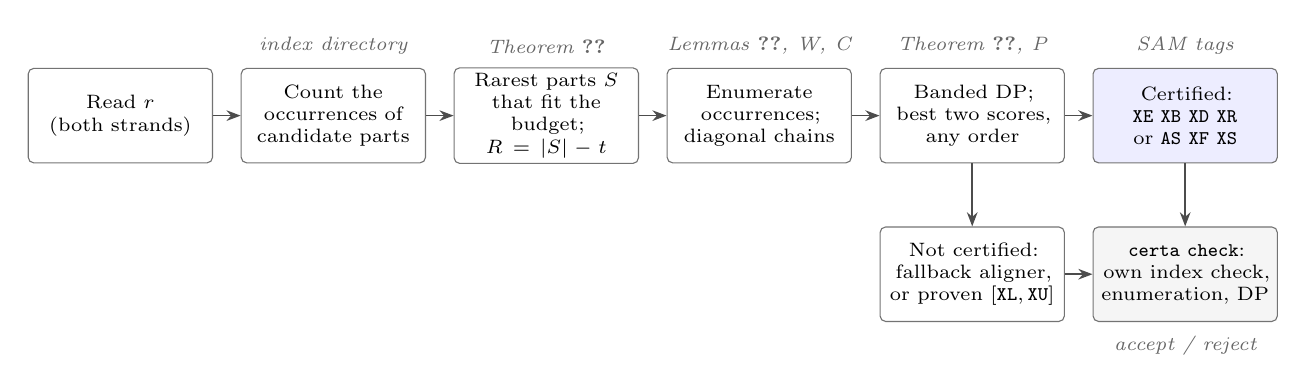
\begin{tikzpicture}[
  box/.style={draw=black!55, rounded corners=2pt, align=center, font=\scriptsize,
              inner sep=2pt, minimum height=12mm, text width=22mm},
  arr/.style={-{Stealth[length=1.8mm]}, black!70, semithick},
  lab/.style={font=\scriptsize\itshape, text=black!60, align=center}]
\node[box] (read) {Read $r$\\(both strands)};
\node[box, right=3.5mm of read] (count) {Count the\\occurrences of\\candidate parts};
\node[box, right=3.5mm of count] (pick) {Rarest parts $S$\\that fit the budget;\\$R=|S|-t$};
\node[box, right=3.5mm of pick] (enum) {Enumerate\\occurrences;\\diagonal chains};
\node[box, right=3.5mm of enum] (dp) {Banded DP;\\best two scores,\\any order};
\node[box, right=3.5mm of dp, fill=blue!7] (cert) {Certified:\\\texttt{XE XB XD XR}\\or \texttt{AS XF XS}};
\node[box, below=8mm of dp] (unc) {Not certified:\\fallback aligner,\\or proven $[\texttt{XL},\texttt{XU}]$};
\node[box, below=8mm of cert, fill=black!4] (check) {\texttt{certa check}:\\own index check,\\enumeration, DP};
\foreach \a/\b in {read/count, count/pick, pick/enum, enum/dp, dp/cert} \draw[arr] (\a) -- (\b);
\draw[arr] (dp) -- (unc);
\draw[arr] (cert) -- (check);
\draw[arr] (unc) -- (check);
\node[lab, above=0.5mm of count] {index directory};
\node[lab, above=0.5mm of pick] {Theorem~\ref{thm:pigeon}};
\node[lab, above=0.5mm of enum] {Lemmas~\ref{lem:L}, W, C};
\node[lab, above=0.5mm of dp] {Theorem~\ref{thm:L}, P};
\node[lab, above=0.5mm of cert] {SAM tags};
\node[lab, below=0.5mm of check] {accept / reject};
\end{tikzpicture}
\caption{Overview. For each read CERTA counts its candidate parts'
occurrences from the index directory, picks the rarest parts that fit a
hit budget (which fixes the certified radius), enumerates their
occurrences, groups them into clusters or chains of diagonals, and
verifies these by banded DP in any order. If the best alignment beats every
bound, the read is certified and its record carries the proof's key
quantities; otherwise it goes to a fallback aligner or, in interval mode,
gets a proven interval. An independent checker re-derives every claim from
the record's witness parts.}
\label{fig:overview}
\end{figure}

\subsection{Objectives}

The reference $G$ is the concatenation of the contigs, separated by runs
of \texttt{N}. A read $r$ of length $L$ is aligned on both strands. An
\texttt{N} in the read or the reference never matches.

\textbf{Edit distance.} $d(r,\ell)$ is the semi-global unit-cost edit
distance of the whole read at locus $\ell$. Tiers S0 (exact, $d=0$) and S1
($1\le d\le R$) certify the minimum of $d$ over the genome.

\textbf{Local score.} BWA-MEM's default scores define
\[
\sigma(A) = \#\text{matches} - 4\cdot\#\text{mismatches}
 - \sum_{\text{gap runs}} (6 + \text{length}) - 5[x>0] - 5[y<L]
\]
for an alignment $A$ of the read span $[x,y)$, so clipped ends cost 5
each. $\OPT(r)$ is the maximum of $\sigma$ over all alignments, both
strands, all of $G$. The \emph{loss} of $A$ is
$\lambda(A) = (y-x) - \sigma(A) - 5[x>0] - 5[y<L]$. Event by event,
$\lambda$ charges 5 per mismatch, $6+2k$ per insertion run of $k$ bases
and $6+k$ per deletion run of $k$ bases; matches cost nothing.

\textbf{Parts and diagonals.} Parts are disjoint read intervals. A part
\emph{occurs exactly} in $A$ when all its bases are matches with no
deletion between them, so $A$ maps it unchanged at one \emph{diagonal}
(reference position minus read position).

\textbf{Index.} The index stores every \texttt{N}-free $q$-mer of $G$ that
starts at a multiple of $s$ ($q=22$, $s=1$ in all experiments: \IdxEntries~G
entries for GRCh38). Every occurrence of a part of length $\ge q+s-1$ is
then found, exactly once, by looking up its $q$-mer at each of $s$ offsets
(Lemma~I in the supplement).

\subsection{The adaptive pigeonhole certificate}\label{sec:pigeon}

\begin{theorem}[Lossless enumeration, adaptive radius]\label{thm:pigeon}
Let $S$ be any set of disjoint parts, each of length $\ge q+s-1$, with all
their occurrences enumerated, and let $t\ge1$. Every locus $\ell$ with
$d(r,\ell)\le |S|-t$ has at least $t$ parts of $S$ occurring exactly at
$\ell$, each on a diagonal within $\pm d(r,\ell)$ of $\ell$'s start
diagonal.
\end{theorem}
\begin{proof}
An edit touches at most one part, so $d$ edits leave at least
$|S|-d\ge t$ parts untouched, and each occurs exactly. Its diagonal differs
from the start diagonal by the number of indels before it, at most $d$.
\end{proof}

The theorem holds for \emph{any} choice of $S$. CERTA therefore counts each
candidate part's occurrences from the index directory, which costs one
range lookup and enumerates nothing, and picks the rarest parts whose
total fits a hit budget. The certified radius $R=|S|-t$ adapts per read: a
read with one repetitive part loses one unit of radius instead of its
certificate. Fixed pigeonhole filters, which split the read into
$k+1$ fixed parts \citep{navarro2001guided}, fail as soon as one part is
repetitive. On all HG002 reads, fixed parts with $k=2$ certify \SeCertFixed\%;
the adaptive choice certifies \SeCert\%. With $t=2$, the $q$-gram threshold
\citep{ukkonen1992qgram}, clusters supported by a single part are skipped
without loss, which makes large budgets affordable.

The same argument allows parts that are searched with one edit. Every
reference $q$-mer within one edit of a read $q$-mer is one of at most
$1+11q$ neighbours, which can be looked up directly. A locus within
$2|S|-1$ edits leaves some part of $S$ with at most one edit, so the radius
becomes $R=2|S|-1$ (Theorem~A in the supplement). The optional pass~V uses
this. Per read it chooses the rarest disjoint $q$-mers by dynamic
programming over read offsets, then, for reads still uncertified, $q$-mers
searched with one edit, up to a radius of 12. Pass~V's records carry no
witness for the independent checker yet.

Clusters of candidate diagonals are verified by banded edit-distance DP
over their diagonals $\pm 2R$, which finds $d(r,\ell)$ exactly for every
locus within $R$ whose witness part lies in the cluster. They are evaluated
in any order, keeping the two smallest distances $b_1\le b_2$ and pruning
each cluster at $b_2-1$. The final $b_1$ is the genome-wide minimum, and,
when $b_1<b_2\le R$, $b_2$ is the exact second-best distance; neither
depends on the evaluation order. A certified read reports the minimum
(\samtag{XE}), whether it is unique or tied (\samtag{XB}), the second best within
the radius (\samtag{XD}) and the radius (\samtag{XR}). A read with two distinct
exact full-length matches is a certified repeat (tier SR): $d_1=0$ with at
least two optimal loci, under any scoring, so MAPQ~0 is proven.

\subsection{The loss lemma and certified local alignment}\label{sec:loss}

Edit distance is not the score that variant callers see. The bridge to
BWA-MEM's objective is a lower bound on the loss.

\begin{lemma}[Loss]\label{lem:L}
Let the parts be disjoint, each of length at least 3, and let $N(A)$ be
the parts inside $A$'s span that do not occur exactly in $A$. Then
$\lambda(A)\ge 5\,|N(A)|$.
\end{lemma}
\begin{proof}[Proof sketch]
Charge each event's cost to the parts it touches. A mismatch lies in one
part and costs 5. A deletion run lies between two consecutive read bases,
so it touches at most one part, and costs at least 7. An insertion run of
$k$ bases that touches $j\ge2$ parts covers the $j-2$ parts between its
first and last, so $k\ge 2+3(j-2)$ and $6+2k\ge 5j$. Every part in $N(A)$
is touched by some event and receives at least 5.
\end{proof}

The length condition is sharp: with parts of length 2, a 4-base insertion
over three parts costs $14<15$. Two consequences make the lemma usable.
First, an alignment with fewer than $t$ exactly occurring parts of $S$ scores at
most
\[
U_t = \max_{[x,y)} \Bigl( (y-x) - 5\max\bigl(0, \#\{\text{parts of } S
\text{ inside } [x,y)\} - t + 1\bigr) - 5[x>0] - 5[y<L] \Bigr),
\]
and for parts of length $\ge 5$ the full span attains the maximum
(Lemma~S in the supplement), so $U_t = L - 5(|S|-t+1)$. Second, a gap run
of $k$ costs at least $6+k$, so an alignment scoring above $b$ has gap
total at most $\pad(b)=\max(0, L-b-7)$ (Lemma~W). Its exact parts then lie
on diagonals within $\pad(b)$ of each other: sorting all occurrences by
diagonal and splitting where consecutive diagonals differ by more than
$\pad(b)$ yields \emph{chains}, and every such alignment lies in one chain
$C$, within $\pm\pad(b)$ of its diagonals, and scores at most $\ub(C)$, the
bound $U$ with $C$'s parts treated as free (Lemma~C).

\begin{theorem}[Certified local optimum, tier SL]\label{thm:L}
Let $\mathit{floor}=U_t$. Evaluate, in any order, every chain with
$\ub>\mathit{floor}$ by banded affine DP \citep{gotoh1982} over its
diagonals $\pm\pad(\mathit{floor})$, keeping the best two scores
$s_1\ge s_2$ (initially $\mathit{floor}$) and skipping chains with
$\ub\le s_2$. If $s_1>\mathit{floor}$ then $\OPT(r)=s_1$.
\end{theorem}
\begin{proof}
An alignment scoring above $s_1$ has at least $t$ exact parts (otherwise it
scores at most $\mathit{floor}$) and a gap total within the pad, so it
lies in some chain $C$. If $C$ was evaluated, the DP saw it. If $C$ was
skipped, it scores at most $\ub(C)\le s_2\le s_1$.
\end{proof}

\textbf{Pairs (tier PR).} The paired objective is $\sigma(A_1)+\sigma(A_2)$
over \emph{proper} pairs: opposite strands, and the reverse mate's first
aligned base 0 to $D$ bases after the forward mate's ($D=850$). A pair with
no exact part in either mate scores at most $U_1+U_2$. Otherwise one mate
lies in one of its chains (an \emph{anchor}), and its partner starts in
that chain's insert window. The window is about 1~kb, so the partner's
short parts (about 12 bases) are searched directly in the reference, with
no index, and Lemma~\ref{lem:L} bounds every partner not found. Anchors are
evaluated best bound first. When the best pair realized exceeds every
remaining bound, it is the maximum pair score over the whole reference
(Theorem~P in the supplement). The largest remaining bound, $S_2$, bounds
every proper pair that differs in some mate and drives a BWA-MEM-style pair
MAPQ.

\subsection{Interval output and an independent checker}\label{sec:intervals}

A read that is not certified still has proven bounds. In interval mode
(\texttt{certa map -{}-intervals}) every record carries $[\samtag{XL},\samtag{XU}]$,
an interval that contains $\OPT$: \samtag{XL} is the score of a shown
alignment and \samtag{XU} is a Lemma~\ref{lem:L} bound together with an
exhaustive search of the chains above it. A record also carries \samtag{XQ},
a certified lower bound of BWA-MEM's single-end MAPQ formula, valid
because the formula is monotone in the best and second-best scores
(Proposition~Q). Nothing goes to a fallback mapper.

\texttt{certa check} verifies these records. It shares no alignment,
bound or lookup code with the mapper. It first validates the index against
the FASTA (every entry's key equals the reference $q$-mer at its position,
no position repeats, and the count equals the number of sampled
\texttt{N}-free $q$-mers), which makes enumeration complete. For each
claimed bound it then recomputes Lemma~\ref{lem:L} from the witness parts
written in the record, enumerates their occurrences itself, rebuilds the
chains and searches them with its own banded DP. A record is accepted only
if every claim follows (Theorem~V in the supplement); pair claims are
re-derived from both mates' records.

\subsection{Long reads}\label{sec:long}

For a long read the parts are no longer a fixed tiling. Let $F_\tau$ be the
read intervals that occur at most $\tau$ times in the reference. Scanning
left to right and taking at each position the shortest interval of
$F_\tau$ that starts there gives the maximum number of disjoint parts
(Theorem~G): $F_\tau$ is closed under extension, so this is interval
scheduling by earliest end. Lemma~\ref{lem:L} needs only disjoint parts of
length $\ge3$, so stretches of the read that no part covers are simply not
charged.

\begin{corollary}[Long-read certificate]\label{cor:long}
Let $lb$ be the score of any known alignment (here minimap2's), with
$lb>U_1$. Build chains with $\pad=L-lb-7$ and evaluate by banded DP every
chain whose bound exceeds the best score so far. Then $\OPT$ is the larger
of $lb$ and the best DP score.
\end{corollary}

A known alignment narrows the band to a few hundred diagonals even for a
15~kb read, so the certificate costs about one banded DP per read. Reads
that span a structural variant fit better under a \emph{split}
objective, in which an alignment is a chain of pieces and each jump between
pieces costs $P$. Lemma~\ref{lem:L} bounds it piecewise. Its certificate
(Theorem~L-J) evaluates chains in rounds. Each round computes exact
prefix and suffix values of the chains evaluated so far, bounds every
unevaluated chain through them, and raises $lb$ to the best alignment
already realized. The rounds end when no unevaluated chain can beat $lb$.

\subsection{Implementation}

\textbf{Short reads.} The index (\texttt{.cidx}) holds the sorted
$(q\text{-mer}, \text{position})$ entries with a bucket directory, and is
memory-mapped. On the GPU, one CUDA thread maps one read with the same
code as the CPU path: counting, part choice, enumeration within a budget
of 16 hits per strand, clustering and banded verification. This first pass
is uniform and fast. The reads it cannot certify are compacted into a
second pass with a budget of 256 hits, so the expensive work stays among
the hard reads. Without a GPU the same passes run on the CPU. A complete
mapping comes in two configurations: uncertified reads either stream
through a pipe into a conventional aligner (minibwa in all experiments),
which runs concurrently, or, in interval mode, get CERTA's own placement
with a proven interval (Section~\ref{sec:intervals}). The next batch is
read and parsed on several threads while the current one maps. With a GPU,
the GPU passes of one batch overlap the CPU passes and formatting of the
previous one; without a GPU, every pass of a batch runs on one small chunk
of reads after another, the threads taking chunks in turn, so that the
slow reads of a pass never leave the other cores waiting at its end. Each
output is written by its own thread. The reported CIGAR is the affine-optimal
alignment at the certified locus. Output is byte-identical across CPU and
GPU, x86-64 and ARM64, and any thread count.

\textbf{Vectorized banded DP.} One row of the Gotoh recurrence is computed
$W$ cells at a time ($W=4$ with NEON or SSE, $8$ with AVX2; 8 lanes of 16
bits for short reads). Inside the row, the deletion state is the only
sequential dependency. With $h_0[b]$ the best of match and insertion and a
gap extension of 1, it unrolls to
\[
H[b] = \max\Bigl(h_0[b],\; \max_{b'\le b}\bigl(h_0[b']+b'\bigr) - b - 6\Bigr),
\]
because taking $b'=b$ adds $h_0[b]-6$, which never wins. This is an
inclusive prefix maximum: $\log_2 W$ in-register shifts per vector and a
carry between vectors. For long reads the DP is also pruned: a cell whose
value plus the number of read bases after it cannot exceed $lb$ is dead,
and once no new piece can start, each row is restricted to the previous
row's live range. The other band DPs use the same devices on the CPU: the
edit-distance band of the end-to-end certificate takes the minimum form
of the identity, on 16-bit lanes or, with every value capped at the limit
plus one (which leaves the result unchanged, since the recurrence is
monotone), on 8-bit lanes; the score-only band of the pair window may stop
once no cell can still beat the threshold its caller needs; and the
traceback fill runs on 16-bit lanes, its sentinels shifted but every
comparison unchanged. Index lookups are batched and prefetched, across a
read's parts and across consecutive reads, and so are the reference bytes
of the repeat copies that tier R compares with the read.

\subsection{Verification of the implementation}\label{sec:verify}

A proof covers the algorithm; the code needs its own evidence. We use four
layers. The oracle tests and lemma checks run in continuous integration on
x86-64 and ARM64, and the Lean proofs are re-checked on every push.
\begin{itemize}
\item \textbf{Brute-force oracles} on synthetic genomes with diverged
  repeat copies, a 50-copy exact repeat, tandem repeats and \texttt{N}
  runs: Sellers' DP \citep{sellers1980} over the entire reference for edit
  distance, a full Gotoh DP of the local objective on both strands, and the
  best proper pair from per-start local scores. Every certificate on every
  seed must match the oracle.
\item \textbf{Exhaustive checks of the finite lemmas}: Lemma~\ref{lem:L} on
  \VlL{} transcript--layout pairs, the one-mismatch variant (Lemma~H) on
  \VlH{}, the edit-to-score bound (Lemma~E) on \VlE{} clipped transcripts,
  and Lemma~S on \VlS{} cases. The checks of Lemmas~\ref{lem:L}, H and S
  also find counterexamples just below their part-length conditions, so
  those conditions are necessary.
\item \textbf{Mutation testing} \citep{jia2011mutation}: \MutTotal{}
  injected faults, each weakening one bound or step in the source. The
  test suite kills \MutKilled; the other \MutEquiv{} are proven to change
  no claim on any input.
\item \textbf{Mechanized proofs} in Lean~4 \citep{demoura2021lean4},
  without external libraries: \LeanTheorems{} theorems in
  \LeanModules{} modules (\LeanLines{} lines). They cover
  Lemma~\ref{lem:L} for transcripts of any length, the edit-to-score bound,
  Lemmas~S and~W, the geometric core of Lemma~C, Theorem~G, the long-read
  pruning and the identity behind the vectorized DP row. Continuous
  integration fails if any of them depends on an unproven assumption
  (\texttt{sorryAx}) or a non-standard axiom.
\end{itemize}

% =====================================================================
\section{Results}

\subsection{Data and setup}

Short reads are GIAB HG002 \citep{zook2016giab} sequenced on a NovaSeq~X
(SRR37356339, \PePairs{} pairs of 150~bp, 44$\times$), and HG001 and HG005
on a NovaSeq~6000 (PRJNA734598; 2$\times$151~bp, \PeReadsMHGOne~M and
\PeReadsMHGFive~M reads). Single-end experiments use R1 only. Timing uses a
seeded random sample of \BenchReads{} reads or pairs, and the provable-error
analysis its first 2~M reads. Long reads are \LrReads{} HG002 PacBio HiFi
reads \citep{wenger2019hifi} (median length \LrMedLen~bp, about 1$\times$).
The reference is the Ensembl GRCh38 primary assembly
\citep{schneider2017grch38}. Unless stated otherwise, runs used galaxy, a
machine with a 128-core Ampere Altra (ARM64) CPU and an NVIDIA A100 80GB.
CPU-only timings were also taken on a2, with four Intel Xeon Gold 5218
CPUs (x86-64, 64 cores in four NUMA nodes) and no GPU. Every pipeline got
64 cores (on galaxy, cores 0--63 under \texttt{taskset}; on a2, with memory
interleaved over the four nodes by \texttt{numactl}, without which the
kernel's page migrations made about half of the runs of one pipeline 1.5
times slower), and all of a host's timings come from one session. Wall times are medians of three
runs after a warm-up (paired BWA-MEM2: one run), with SAM written to
\texttt{/dev/null}. All tools ran with default settings, except the batch
size of minibwa when it is CERTA's fallback (Section~\ref{sec:speed}).

\subsection{Certification}\label{sec:cert}

In single-end mode CERTA certifies \SeCert\% of all \SeReads{} reads:
\SeExact\% are exact, \SeEdits\% within the radius, and \SeRepeat\%
certified repeats (Fig.~\ref{fig:cert}). In paired mode, the pair
certificate adds \PeCertPR\% of reads, and \PeCert\% of the \PeReads{}
reads are certified. The NovaSeq~6000 samples, with 151~bp reads and more
sequencing errors, reach \PeCertHGOne\% (HG001) and \PeCertHGFive\%
(HG005). The uncertified reads are mostly limited by repeats (fewer parts
fit the budget, so the floor is close to $L$) or lose too much: with
$q=22$ a 150~bp read has at most six disjoint parts, and
Lemma~\ref{lem:L} charges 5 points per part, so no exact-part certificate
can prove an alignment that loses 30 points or more. Full certification
(\texttt{-{}-full-cert}) moves this limit on the main index alone. It
raises the hit budget to 4096 per strand (pass~3), adds the certified local
tier, and adds pass~V's adaptive and one-edit parts. On the first 2~M
HG002 reads it certifies \SlSeFcCert\% single-end and \SlPeFcCert\% of
paired reads, against \SlSeDefCert\% and \SlPeDefCert\% by default and
\SlSeNoVCert\% single-end without pass~V. A second, $q=15$ index
(\texttt{-{}-index2}) adds little on top of that (\SlSeIxCert\%) for a
second 23~GB index (Section~\ref{sec:slow}).

\begin{figure}[t]
\centering
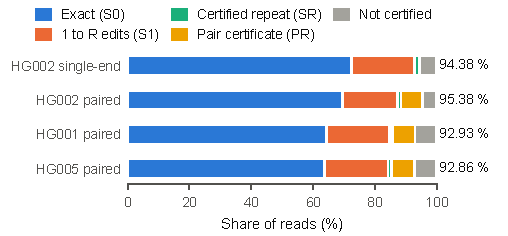
\includegraphics{figures/certification.pdf}
\caption{Share of reads certified, by certificate type. HG002 single-end:
all \SeReads{} R1 reads; paired: all reads of each sample. S0, exact
match; S1, between 1 and $R$ edits; SR, a proven exact repeat; PR, the
proper-pair certificate. The uncertified reads are mapped by the fallback
aligner, or bounded by an interval in interval mode.}
\label{fig:cert}
\end{figure}

\subsection{Provable errors of heuristic aligners}\label{sec:errors}

A certificate turns disagreement with CERTA into a provable error. For
the \WkReads{} certified reads of the 2~M sample we rescored every other
aligner's alignment from its CIGAR and NM under BWA-MEM's scores, so each
tool is judged on the same scale (Table~\ref{tab:errors}). Every tool
places some reads at another locus whose alignment scores at least one
edit (5 points) below CERTA's alignment at the certified locus.
BWA-MEM2 does so for \WkBwaMiss{} reads (\WkBwaMissPct\%), which
extrapolates to about \WkBwaPerGenome{} provably misplaced reads among the
certified reads of one 22$\times$ genome. minibwa makes
\WkMiniOverBwa$\times$ as many errors, and strobealign
\WkStrobeOverBwa$\times$. strobealign also gives MAPQ~$\ge 20$ to
\WkStrobeTies{} reads (\WkStrobeTiesPct\% of the \WkTies{} proven ties)
that occur in two or more identical copies, a placement that is right by
chance in at most half the cases. strobealign, minimap2 and Bowtie~2
leave reads unmapped although an alignment with at most five edits exists. Among the
heuristic tools, errors grow with speed (Fig.~\ref{fig:errors}). Rabema
\citep{holtgrewe2011rabema} defines errors against an edit-distance gold
standard computed by a fully sensitive mapper. Here the reference point is
a per-read proof, and errors are scored under BWA-MEM's own objective.

\begin{table}[t]
\centering
\caption{Provable errors on \WkReads{} certified HG002 reads (2~M
sample). \emph{Misplaced}: placed at another locus, whose alignment scores
at least 5 points (one edit) below CERTA's alignment at the certified
locus, all scored under BWA-MEM's scheme. \emph{Unmapped}: no alignment reported although one
with at most five edits exists. \emph{Ties}: reads proven to occur in at
least two identical copies, given MAPQ $\ge 20$ (of \WkTies{}).}
\label{tab:errors}
\small
\begin{tabular}{@{}lrrrr@{}}
\toprule
Aligner & Misplaced & of which MAPQ $\ge 20$ & Unmapped & Ties, MAPQ $\ge 20$\\
\midrule
BWA-MEM2 2.3 & \WkBwaMiss{} (\WkBwaMissPct\%) & \WkBwaQ & \WkBwaUnmapped & \WkBwaTies\\
minibwa 0.7 & \WkMiniMiss{} (\WkMiniMissPct\%) & \WkMiniQ & \WkMiniUnmapped & \WkMiniTies\\
strobealign 0.18 & \WkStrobeMiss{} (\WkStrobeMissPct\%) & \WkStrobeQ & \WkStrobeUnmapped & \WkStrobeTies\\
minimap2 2.31 \texttt{-x sr} & \WkMmMiss{} (\WkMmMissPct\%) & \WkMmQ & \WkMmUnmapped & \WkMmTies\\
Bowtie~2 2.5.5 & \WkBtMiss{} (\WkBtMissPct\%) & \WkBtQ & \WkBtUnmapped & \WkBtTies\\
\midrule
CERTA, certified reads & 0 & 0 & 0 & 0\\
\bottomrule
\end{tabular}
\end{table}

\begin{figure}[t]
\centering
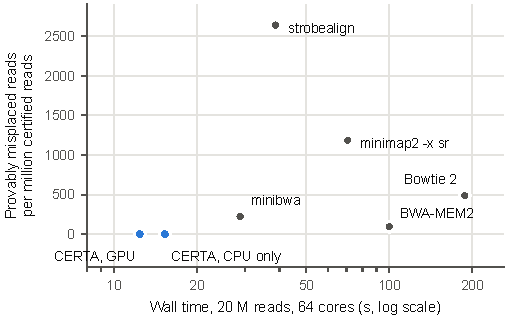
\includegraphics{figures/errors_vs_speed.pdf}
\caption{Provable misplacements against wall time, single-end, 20~M
HG002 reads on galaxy's 64 cores (Table~\ref{tab:speed}; one session).
CERTA: its fastest complete configuration on CPU alone and with the A100;
certified reads make no provable error by construction. Error counts as in
Table~\ref{tab:errors}.}
\label{fig:errors}
\end{figure}

\subsection{Speed}\label{sec:speed}

Every pipeline was timed in one session per host, on the same 64 cores (on
galaxy, which has 128, every pipeline ran under \texttt{taskset} on cores
0--63), mapping \BenchReads{} reads or pairs with SAM written to
\texttt{/dev/null} (Table~\ref{tab:speed}). CERTA runs in two complete
configurations. \emph{With a fallback}, it streams the reads it cannot
certify into minibwa, which maps them concurrently; each starts 64
threads on the 64 cores. \emph{In interval mode} it maps every read
itself: a certified read gets its optimum, any other read a proven interval
around its optimum (Section~\ref{sec:check}), and nothing goes to another
aligner. With or without the GPU, CERTA certifies the same reads
(\CpuTierCert\% of the 20~M single-end reads, on both hosts) and writes the
same bytes.

Single-end, every default CERTA configuration is faster than every other
aligner on both hosts. On CPU alone, interval mode takes \FGSCpuIvWall~s on galaxy and
\FASCpuIvWall~s on a2: \FGSCpuIvXMini$\times$ and \FASCpuIvXMini$\times$
faster than minibwa, the fastest of the other aligners, and
\FGSCpuIvXBwa$\times$ and \FASCpuIvXBwa$\times$ faster than BWA-MEM2. With
the A100 it takes \FGSGpuIvWall~s (\FGSGpuIvXMini$\times$ minibwa,
\FGSGpuIvXBwa$\times$ BWA-MEM2).

Paired, interval mode is again the fastest: \FGPCpuIvWall~s on galaxy's
CPU and \FAPCpuIvWall~s on a2's (\FGPCpuIvXMini$\times$ and
\FAPCpuIvXMini$\times$ minibwa; \FGPCpuIvXBwa$\times$ and
\FAPCpuIvXBwa$\times$ BWA-MEM2), and \FGPGpuIvWall~s with the A100
(\FGPGpuIvXMini$\times$ minibwa, \FGPGpuIvXBwa$\times$ BWA-MEM2). With the
fallback, a pair with an uncertified mate goes to minibwa whole, so that it
can be paired; these pairs cost minibwa several times its average pair,
and the pipeline takes \FGPCpuKtWall~s on galaxy's CPU and
\FAPCpuKtWall~s on a2's (\FGPCpuKtXMini$\times$ and \FAPCpuKtXMini$\times$
minibwa), and \FGPGpuKtWall~s with the A100 (\FGPGpuKtXMini$\times$).

Full certification costs time. At full scale it certifies \FCCertSFc\% of
single-end reads and \FCCertPFc\% of paired reads, against \FCCertSDef\%
and \FCCertPDef\% by default, the same on both hosts and with the A100. On
galaxy's CPU it takes \FCGSFcCpuWall~s single-end and \FCGPFcCpuWall~s
paired (Table~\ref{tab:speed}). That is slower than minibwa, but
\FCGSFcCpuXBwa$\times$ and \FCGPFcCpuXBwa$\times$ faster than BWA-MEM2.
Most of the difference from the default is pass~V: without it, full
certification takes \FCGSNoVCpuWall~s and \FCGPNoVCpuWall~s and certifies
\FCCertSNoV\% and \FCCertPNoV\%. Peak memory is
the same as by default: \MemSOld~GiB single-end and \MemPOld~GiB paired
for the build timed in Table~\ref{tab:speed}. The current build releases
input pages once they are parsed and holds the index directory in 32
bits. That brings peak memory to \MemSNew~GiB and \MemPNew~GiB on the
CPU (\MemSGpuNew~GiB and \MemPGpuNew~GiB with the A100), with identical
output, and it is up to \MemFasterMax\% faster.

Five changes, none of which changes any output, made the CPU pipelines
fast. Every pass of a batch runs on one chunk of 64 reads after another,
the threads taking chunks in turn, so the slow reads of one pass (tier R's
repeats above all) no longer hold the other cores at its end. The next
batch is parsed on several threads while the current one maps, and each
output is written by its own thread. The edit-distance band, the
score-only band and the traceback fill run on 8- to 16-bit vector lanes
(exact for every input; supplement). Index lookups, and tier R's reads of
the reference at each repeat copy, are prefetched, and the search for
copies of tier R's alignment reuses the read's own lookups. And the fallback
minibwa takes 10-Mbp batches (\texttt{-K 10m}): with its default
(100~Mbp--1~Gbp), its threads waited on a few slow reads per batch of
CERTA's hard reads, and the paired pipeline on a2 spent \FAPCpuKdSys~s in
the kernel instead of \FAPCpuKtSys~s and took \FAPCpuKdWall~s.
Single-end, \texttt{-K} changes nothing in minibwa's output. On pairs it
changes the per-batch insert-size estimate, and with it \KbatchDiffRecords{}
of HG005's chromosome-20 records, but no F1 of
Table~\ref{tab:f1}'s callers in the fourth decimal (SNVs and indels, GATK
and bcftools).

\begin{table}[t]
\centering
\caption{Wall time (s) to map \BenchReads{} HG002 reads (single-end) or
pairs (paired) completely, every pipeline on 64 cores, and in parentheses
the speed relative to minibwa (minibwa's time over the pipeline's). One
session per host; medians of \FReps{} runs (paired BWA-MEM2: one run).
\emph{galaxy}: a 128-core Ampere Altra (ARM64), pipelines pinned to cores
0--63; the A100 rows also use one NVIDIA A100. \emph{a2}: four Intel Xeon
Gold 5218 (x86-64, 64 cores, four NUMA nodes), no GPU, every pipeline's
memory interleaved over the nodes. CERTA + minibwa:
CERTA streams its uncertified reads into minibwa; interval mode: no
fallback (every read certified or given a proven interval). The full
certification rows come from a later session with the same protocol, whose
default rows reproduce this table's interval rows within 1~s.}
\label{tab:speed}
\small
\begin{tabular}{@{}lllll@{}}
\toprule
& \multicolumn{2}{c}{galaxy (ARM64)} & \multicolumn{2}{c}{a2 (x86-64)}\\
\cmidrule(lr){2-3}\cmidrule(l){4-5}
Pipeline & single-end & paired & single-end & paired\\
\midrule
BWA-MEM2 & \FGSBwaWall{} (\FGSBwaXMini) & \FGPBwaWall{} (\FGPBwaXMini) & \FASBwaWall{} (\FASBwaXMini) & \FAPBwaWall{} (\FAPBwaXMini)\\
minibwa & \FGSMiniWall{} (1.00) & \FGPMiniWall{} (1.00) & \FASMiniWall{} (1.00) & \FAPMiniWall{} (1.00)\\
strobealign & \FGSStrobeWall{} (\FGSStrobeXMini) & -- & \FASStrobeWall{} (\FASStrobeXMini) & --\\
minimap2 \texttt{-x sr} & \FGSMmWall{} (\FGSMmXMini) & -- & \FASMmWall{} (\FASMmXMini) & --\\
Bowtie~2 & \FGSBtWall{} (\FGSBtXMini) & -- & \FASBtWall{} (\FASBtXMini) & --\\
\midrule
CERTA + minibwa, CPU only & \FGSCpuWall{} (\FGSCpuXMini) & \FGPCpuKtWall{} (\FGPCpuKtXMini) & \FASCpuWall{} (\FASCpuXMini) & \FAPCpuKtWall{} (\FAPCpuKtXMini)\\
CERTA interval mode, CPU only & \FGSCpuIvWall{} (\FGSCpuIvXMini) & \FGPCpuIvWall{} (\FGPCpuIvXMini) & \FASCpuIvWall{} (\FASCpuIvXMini) & \FAPCpuIvWall{} (\FAPCpuIvXMini)\\
CERTA + minibwa, A100 & \FGSGpuWall{} (\FGSGpuXMini) & \FGPGpuKtWall{} (\FGPGpuKtXMini) & -- & --\\
CERTA interval mode, A100 & \FGSGpuIvWall{} (\FGSGpuIvXMini) & \FGPGpuIvWall{} (\FGPGpuIvXMini) & -- & --\\
\midrule
\multicolumn{5}{@{}l}{\emph{Full certification (\texttt{-{}-full-cert}), interval mode}}\\
CPU only & \FCGSFcCpuWall{} (\FCGSFcCpuXMini) & \FCGPFcCpuWall{} (\FCGPFcCpuXMini) & \FCASFcCpuWall{} (\FCASFcCpuXMini) & \FCAPFcCpuWall{} (\FCAPFcCpuXMini)\\
A100 & \FCGSFcGpuWall{} (\FCGSFcGpuXMini) & \FCGPFcGpuWall{} (\FCGPFcGpuXMini) & -- & --\\
\bottomrule
\end{tabular}
\end{table}

\subsection{Against fully sensitive mappers}\label{sec:slow}

Lossless $k$-error mappers find every alignment within a fixed error
limit. We ran Yara 1.0.5 (from SeqAn, \url{https://github.com/seqan/seqan})
with \texttt{-e 4 -y full}, every alignment with at most 4\% errors (6 edits
at 150~bp), and RazerS~3 \citep{weese2012razers3} with \texttt{-i 96 -rr
100}, 100\% recognition of matches with at least 96\% identity. Each ran on
the same 64 cores of galaxy as CERTA's interval mode on the CPU
(Table~\ref{tab:slow}). Full certification takes \SlSeFcWall~s for 2~M
single-end reads; Yara takes \SlSeYaraWall~s (\SlSeYaraX$\times$), and
\SlPeYaraX$\times$ CERTA's time on pairs. RazerS~3 needs \SlRazWall~s for
the first 200,000 reads, against \SlRazCertaWall~s (\SlRazX$\times$), and
its paired mode aborted for lack of memory. The two guarantees differ in
scope. Yara and RazerS~3 cover every read up to their error limit, but
only end-to-end alignments. CERTA's radius adapts per read (up to 12 edits
end to end with pass~V) and its local tier also covers clipped alignments,
but some reads stay uncertified. Within their own error limit, neither tool
misses a read that CERTA certifies. Of the \SlYaraEtoE{} reads that CERTA
certifies end to end, Yara places \SlYaraElse{} of them at a locus with more
edits than the proven minimum. It leaves \SlYaraUnm{} of them unmapped,
\SlYaraUnmWithin{} with a proven distance within 4\% of the read length and
\SlYaraUnmBeyond{} beyond it.
Of the \SlRazEtoE{} such reads among the first 200,000, RazerS~3 leaves
\SlRazEtoEUnm{} unmapped, again all beyond its limit. CERTA certifies these
reads, and the reads that need clipping: of those, Yara leaves
\SlYaraLocalUnmPct\% unmapped and RazerS~3 \SlRazLocalUnmPct\%.

Before pass~V we asked what exhaustive search could add. Full certification
with both indexes then left \HrUncPct\% of the reads (\HrUnc) uncertified.
On these, Yara with \texttt{-e 8} (every alignment within 12 edits) found a
best end-to-end alignment within 6 edits for only \HrLeSixPct\% of all
reads, \HrRepPct{} points of them reads whose parts are too repetitive for
the hit budget. Another \HrSevenElevenPct\% needed 7 to 11 edits, and
\HrNonePct\% had no end-to-end alignment within 12 edits. That search took
\HrYaraWall~s, \HrCpuPerRead~CPU-s per read. Pass~V, with rarer parts and a
radius of up to 12, now certifies most of the first two groups on the main
index alone (\SlSeFcCert\% in all). What remains needs clipped
certificates or larger radii.

\begin{table}[t]
\centering
\caption{CERTA against fully sensitive mappers: share of reads certified
(\%), wall and CPU time (s), 2,000,000 HG002 reads or pairs, galaxy, 64
cores, CPU only. CERTA in interval mode (every read gets a record), median
of three runs; Yara one run. RazerS~3 ran on the first 200,000 reads only
(its paired mode aborted).}
\label{tab:slow}
\small
\begin{tabular}{@{}lrrrrrr@{}}
\toprule
& \multicolumn{3}{c}{Single-end} & \multicolumn{3}{c}{Paired}\\
Mapper and settings & Cert. & Wall & CPU & Cert. & Wall & CPU\\
\midrule
CERTA, default & \SlSeDefCert & \SlSeDefWall & \SlSeDefCpu & \SlPeDefCert & \SlPeDefWall & \SlPeDefCpu\\
CERTA \texttt{-{}-full-cert}, no pass~V & \SlSeNoVCert & \SlSeNoVWall & \SlSeNoVCpu & \SlPeNoVCert & \SlPeNoVWall & \SlPeNoVCpu\\
CERTA \texttt{-{}-full-cert} & \SlSeFcCert & \SlSeFcWall & \SlSeFcCpu & \SlPeFcCert & \SlPeFcWall & \SlPeFcCpu\\
CERTA \texttt{-{}-full-cert -{}-index2} & \SlSeIxCert & \SlSeIxWall & \SlSeIxCpu & \SlPeIxCert & \SlPeIxWall & \SlPeIxCpu\\
Yara \texttt{-e 4 -y full} & -- & \SlSeYaraWall & \SlSeYaraCpu & -- & \SlPeYaraWall & \SlPeYaraCpu\\
\midrule
\multicolumn{7}{@{}l}{\emph{First 200,000 reads}}\\
CERTA \texttt{-{}-full-cert} & \SlRazCertaCert & \SlRazCertaWall & \SlRazCertaCpu & -- & -- & --\\
RazerS~3 \texttt{-i 96 -rr 100} & -- & \SlRazWall & \SlRazCpu & -- & aborted & \\
\bottomrule
\end{tabular}
\end{table}

\subsection{Variant-calling accuracy}

We mapped every read of each sample, kept chromosome 20, called variants
with GATK HaplotypeCaller \citep{poplin2017gatk} and with bcftools
\citep{danecek2021bcftools}, and compared SNVs and indels separately with
rtg vcfeval \citep{cleary2015vcfeval} against the GIAB v4.2.1 benchmark
\citep{wagner2022giab}. The same caller settings were used for both
pipelines. CERTA's F1 is above BWA-MEM2's in \PeVWins{} of
\PeVComparisons{} paired comparisons (Table~\ref{tab:f1}) and in all four
single-end comparisons on HG002 (GATK SNVs \SeVGSCertaF{} against
\SeVGSBwaF; \texttt{certa/FINDINGS.md}, Section~4). In paired mode the gain comes from precision: on
HG002, GATK reports \PeVBGSFpCerta{} false-positive SNVs against
\PeVBGSFpBwa{} for BWA-MEM2, with \PeVBGSFnCerta{} false negatives against
\PeVBGSFnBwa. The one exception is HG001 GATK indels, \PeVAGIDelta{} in F1.

\begin{table}[t]
\centering
\caption{Variant-calling F1 on chromosome 20 against GIAB v4.2.1, paired
reads, CERTA (+ minibwa fallback) / BWA-MEM2, and the difference.}
\label{tab:f1}
\small
\begin{tabular}{@{}llll@{}}
\toprule
Sample & Caller & SNVs & Indels\\
\midrule
\multirow{2}{*}{HG002} & GATK & \PeVBGSCerta{} / \PeVBGSBwa{} (\PeVBGSDelta) & \PeVBGICerta{} / \PeVBGIBwa{} (\PeVBGIDelta)\\
 & bcftools & \PeVBBSCerta{} / \PeVBBSBwa{} (\PeVBBSDelta) & \PeVBBICerta{} / \PeVBBIBwa{} (\PeVBBIDelta)\\
\multirow{2}{*}{HG001} & GATK & \PeVAGSCerta{} / \PeVAGSBwa{} (\PeVAGSDelta) & \PeVAGICerta{} / \PeVAGIBwa{} (\PeVAGIDelta)\\
 & bcftools & \PeVABSCerta{} / \PeVABSBwa{} (\PeVABSDelta) & \PeVABICerta{} / \PeVABIBwa{} (\PeVABIDelta)\\
\multirow{2}{*}{HG005} & GATK & \PeVCGSCerta{} / \PeVCGSBwa{} (\PeVCGSDelta) & \PeVCGICerta{} / \PeVCGIBwa{} (\PeVCGIDelta)\\
 & bcftools & \PeVCBSCerta{} / \PeVCBSBwa{} (\PeVCBSDelta) & \PeVCBICerta{} / \PeVCBIBwa{} (\PeVCBIDelta)\\
\bottomrule
\end{tabular}
\end{table}

\subsection{Interval output and independent checking}\label{sec:check}

In interval mode on all \IvReads{} HG005 reads, \IvExact\% of records are
proven exact ($\samtag{XL}=\samtag{XU}$) with no fallback mapper. Variant-calling
F1 stays above BWA-MEM2's in all \IvVWins{} comparisons (GATK SNVs
\IvVGS{} against \IvVGSBwa). \samtag{XQ}, the certified lower bound of the
MAPQ formula, is not usable as a MAPQ: beyond the radius it bounds the
second-best score by about one point per edit, so reads carrying a SNV get
low \samtag{XQ} and a caller's MAPQ filter drops exactly the variant reads.

The checker accepted all \CkRecords{} honest records of 2~M pairs each of
HG002 and HG005, including \CkXS{} pair claims, at \CkUsLo--\CkUsHi~$\mu$s
of CPU per record, about the mapper's own cost. Validating the index takes
\IdxCheckSec~s once per reference. To test that it rejects false claims, we injected
\CkFaults{} faults of \CkFaultKinds{} kinds that make a record false by
construction (a score raised by one, a clip, a removed witness, a raised
\samtag{XQ}, an interval with $\samtag{XU}<\samtag{XL}$, among others). All
\CkRejected{} were rejected, with no false alarm on untouched records. The
checker also found a real bug: records whose alignment ran off the
circular chrM kept their interval after the alignment was dropped.

\subsection{Long reads}\label{sec:longres}

On the \LrReads{} HiFi reads, a typical alignment loses \LrMedLoss{}
points, while the certificate tolerates a loss up to $L-U_1$, median
\LrMedCeil. The certificate therefore applies to \LrFit\% of reads with
minimap2's alignment as $lb$ (pre-registered criterion: 90\%), and to
\LrProvenPct\% when $lb$ may be its best sub-path.
Corollary~\ref{cor:long} proves $\OPT$ for all \LrProven{} of them. The split certificate adds
\LrJumpProven{} reads that span structural variants, so the optimum is
proven for \LrExactAll\% of reads. For \LrAbovePct\% of the proven reads
$\OPT$ is higher than minimap2's alignment under the same scores. On a
verified subsample of \LrVerifyReads{} reads, a full DP of $\pm$1~kb
around the known locus never exceeded the proven optimum. The remaining
reads are clipped (\LrMissClip\%, mostly split alignments), lose too much
(\LrMissLoss\%, mostly a gap of 500 bases or more), are repeat-limited
(\LrMissRep\%) or unmapped (\LrMissUnm\%).

The certificate costs \LrCpu~s of CPU for the whole sample, against
\LrCpuMm~s for minimap2's mapping and alignment (\LrCpuRatio$\times$;
Fig.~\ref{fig:hifi}). The vectorized DP row, batched index lookups and
pruning to live cells (only \LrCellsPct\% of the band can still beat $lb$)
took the median DP per read from \LrDpMedScalar~ms to \LrDpMed~ms. None of
these changes altered a certificate. Winnowmap2 \citep{jain2022winnowmap2},
built for repetitive references, takes \SlHifiWmWall~s on the same reads
(64 cores, \SlHifiWmIdx~s of it indexing the reference),
\SlHifiWmX$\times$ the \SlHifiCertaWall~s of minimap2 plus the certificate. The split certificate is costlier:
median \LrJumpMedSec~s per attempted read. Of the \LrJumpAttempted{}
attempted reads, \LrJumpInterval{} keep an interval and \LrJumpCapped{}
reach the cell cap, which also leaves an interval.

\begin{figure}[t]
\centering
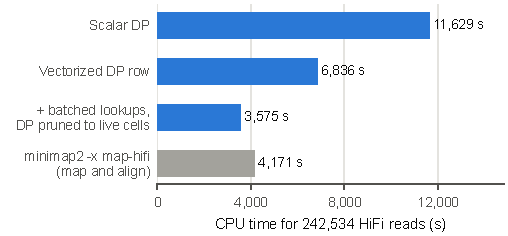
\includegraphics{figures/hifi_cost.pdf}
\caption{CPU time to certify the optimum of \LrReads{} HG002 HiFi reads
(Corollary~\ref{cor:long}; 64 threads), after each optimization, against
minimap2 \texttt{-x map-hifi} mapping and aligning the same reads. Every
version proves the same optima.}
\label{fig:hifi}
\end{figure}

% =====================================================================
\section{Discussion}

Certification changes what an aligner can say about its own output. For
95\% of real short reads CERTA's alignment comes with a proof that no
better alignment exists anywhere in the reference, with the uniqueness of
the optimum, and with the distance to the second best. This makes three
things possible. First, aligners can be evaluated on real data, not only
on simulations: every heuristic aligner we tested misplaces reads that
have a provably better locus, at rates that grow with speed. Second, the
output can be verified by a program that trusts neither the mapper's code
nor its authors. Third, exactness need not cost speed: on CPU alone, and
more so with a GPU, CERTA's default configuration maps reads and pairs
faster than every other aligner we timed, and its variant calls have the
higher F1 than BWA-MEM2's in \PeVWins{} of \PeVComparisons{} comparisons.
Certifying more reads does cost time: full certification (\FCCertSFc\% of
single-end reads) is slower than minibwa, though still
\FCGSFcCpuXBwa$\times$ faster than BWA-MEM2.

The certificate is about the optimization problem, not about the read's
true origin. A read from a diverged copy of a repeat can align better to
another copy. No aligner can resolve that from the read alone, but a
certified read at least shows it: the reported second-best distance says
how close the alternative is.

\textbf{Limitations.} About 5\% of short reads carry no certificate in the
default mode; they get the fallback aligner's alignment, or a proven
interval in interval mode. The S0/S1 tiers certify edit distance, while
callers use the affine alignment at that locus; the certified local tier
(Theorem~\ref{thm:L}) closes this gap but certifies fewer reads. MAPQ
reuses BWA-MEM's formula rather than a calibration from the certified
second best. The fastest configurations add one A100 to the 64 cores, so
cost per genome should be weighed alongside wall time; on CPU alone CERTA
is still the fastest. Accuracy was measured on chromosome 20 of three GIAB
samples for CERTA with its fallback, and of one (HG005) for interval mode,
the fastest paired configuration, and for the paired fallback's 10-Mbp
batches; long reads on one HiFi sample at
1$\times$, with a standalone tool rather than the mapper. The written proofs have not yet been reviewed
by a second person; the mechanized lemmas reduce, but do not remove, that
debt.

\textbf{Outlook.} The limits are measurable. Pass~V runs on the CPU only
and costs about \SlSeFcCpu~CPU-s per 2~M single-end reads against
\SlSeNoVCpu~CPU-s without it; a GPU version, and witnesses for its records
so that the independent checker covers them, are the next steps. A GPU pair
pass and a certificate for the uncertified mate's fallback would raise the
fallback configuration's paired speed. The interval
contract (every read gets either an exact optimum or a proven interval,
and a checker for both) extends naturally to long reads, where a known
alignment already makes the certificate cheaper than mapping.

\section*{Funding}
\textit{To be added.}

\section*{Conflict of interest}
None declared.

\section*{Data availability}
The reads are public: HG002 NovaSeq~X (SRA SRR37356339, BioProject
PRJNA1427896), HG001 and HG005 NovaSeq~6000 (SRR14724533, SRR14724528,
BioProject PRJNA734598), and the GIAB HG002 PacBio HiFi reads. Raw
measurements are in \texttt{certa/bench/results/} of the repository.

\bibliographystyle{plainnat}
\bibliography{refs}

\end{document}
